\documentclass[../Draft_harmonization_paper.tex]{subfiles}

\begin{document}

\section*{Supporting Information}
\label{sec:SI}

\subsection*{Discrepancies in trait definitions}

\begin{landscape}
    \begin{longtable}{m{1.8cm}|m{3cm}|m{3cm}|m{3cm}|m{3cm}|m{3.2cm}|m{3cm}}
        \caption{Comparison of trait definitions between invertebrate trait databases. Only traits that are differently described across databases are listed. The definition is quoted if it enables differences to be identified, otherwise the differences are described. The hyphen indicates a missing trait. Reproduction was captured in multiple grouping features per database. Hence, differences for reproduction have been described in the paper. Body form traits are not different between databases, except that the Vieira database contains the trait Bluff (blocky) which does not appear in the other databases.}
        \label{stab:trait_definitions}
        \endfirsthead
        \toprule[.1em]
        Trait & \specialcell{Freshwater- \\ ecology.info} & Tachet & CONUS & Vieira & Australia & New Zealand \\
        \toprule[.1em]
        Feeding shredder & 
        "Feed from fallen leaves, plant tissues, CPOM" & 
        "Eat coarse detritus, plants or \textit{animal material}" & 
        \begin{itemize}
            \item "Shred decomposing vascular plant tissue"
            \item Trait herbivore includes among others insect that shred \textit{living aquatic plants} 
        \end{itemize} & 
        Shredder & 
        \begin{itemize}
            \item Detrivore \textsuperscript{\textit{a}}
            \item Trait herbivore includes among others the trait shredder
        \end{itemize} & 
        Shredders
        \\ 
        \midrule
        Feeding predator & 
        "Eating from prey" & 
        \begin{itemize}
            \item Carvers, engulfers \& swallowers
            \item Piercers (plants \& animals) are an additional trait
        \end{itemize} & % Notes: Tachet -> Piercer (plants & animals)
        Engulfers ("ingest prey whole or in parts") \& 
        piercers ("prey tissues and suck fluids") & 
        Predator &
        Piercer \& engulfer &
        Predator
        \\ 
        \midrule
        Feeding filter-feeder & 
        Distinguishes between active and passive &
        No distinction between active and passive &
        No distinction between active and passive &
        No distinction between active and passive &
        No distinction between active and passive &
        No distinction between active and passive
        \\
        \toprule[.1em]
        Semivoltine & 
        "One generation in two years" & 
        "Life cycle lasts \textit{at least} two years" & 
        "$< 1$ generation per year" & 
        "$< 1$ generation per year" & 
        "$< 1$ generation per year" & 
        "$< 1$ reproductive cycle per year"
        \\
        \midrule
        Multivoltine & 
        "\textit{Three} or more generations per year" \textsuperscript{\textit{b}}& 
        "Able to complete \textit{at least} two successive generations per year" &
        "$> 1$ generations per year" &
        "$> 1$ generations per year" & 
        \begin{itemize}
            \item 1-2 generations per year
            \item bi/multivoltine
            \item up to 5 generations per year
            \item up to 10 generations per year
        \end{itemize}
        & 
        "$> 1$ reproductive cycles per year"
        \\
        \toprule[.1em]
        Locomotion swimming & 
        \begin{itemize}
            \item Passive movement like floating or drifting (trait swimming/scating)
            \item Active movement (trait swimming/diving)
        \end{itemize}. &
        \begin{itemize}
            \item Surface swimmers (over and under the water surface)
            \item Full water swimmers (e.g. Baetidae).
        \end{itemize} & 
        "Adapted for "fishlike" swimming" & 
        Swimmer & 
        Distinguishes swimmer and skater & 
        Swimmers (water column)
        \\
        \midrule
        Locomotion burrowing & 
        "Burrowing in \textit{soft} substrates or boring in \textit{hard} substrates" & 
        \begin{itemize}
            \item Burrowing "within the first centimeters of the benthic fine sediment"
            \item Differentiates also the trait interstitial (endobenthic)
        \end{itemize} & 
        "Inhabiting \textit{fine} sediment of streams and lakes" &
        Burrower & 
        "Moving deep into the substrate and thus avoiding flow" &
        Burrowers (infauna)
        \\
        \midrule
        Locomotion sprawling \& walking & 
        "Sprawling or walking actively with legs, pseudopods or on a mucus" &
        - & 
        Sprawling: "inhabiting the surface of floating leaves of vascular hydrophytes or fine sediments" & 
        Sprawler &
        - & 
        - \\
        \midrule
        Locomotion crawling & 
        - &
        "Crawling over the bottom substrate" & 
        Defined as crawling on the surface of floating leaves or fine sediments on the bottom & 
        - & 
        Database contains traits crawler, 
        sprawler, climber and clinger. &
        Crawlers (epibenthic) \\
        \midrule
        Locomotion sessil & 
        Does not distinguish temporarily and permanently attached & 
        Distinguishes temporarily and permanently attached & 
        Does not distinguish temporarily and permanently attached & 
        Does not distinguish temporarily and permanently attached & 
        Distinguishes temporarily and permanently attached & 
        Does not distinguish temporarily and permanently attached \\
        \toprule[.1em]
        Respiration plastron \& spiracle & 
        Plastron and spiracle (aerial) are two separate traits & 
        Definition includes respiration using air stores of aquatic plants & 
        Plastron and spiracle combined into one trait & 
        Distinguishes spiracular gills, plastron, atmospheric breathers and plant breathers &
        Plastron and spiracle (termed aerial) occur as separate and combined traits. Contains also traits: air (plants), atmospheric, and functional spiracles &
        Distinguishes plastron and spiracle (termed aerial) \\
        \toprule[.1em]
        Body size small & 
        - &
        \multirow{3}{*}{\specialcell{Multiple size \\ classifications \textsuperscript{\textit{d}}}} & 
        $<$ 9 mm & 
        $<$ 9 mm & 
        $<$ 9 mm \textsuperscript{\textit{a;c}} &
        \multirow{3}{*}{\specialcell{Multiple size \\ classifications \textsuperscript{\textit{e}}}}
        \\
        \cline{1-2}
        \cline{4-6}
        Body size medium & 
        - &
        &
        9 - 16 mm & 
        9 - 16 mm & 
        9 - 16 mm &
        \\
        \cline{1-2}
        \cline{4-6}
        Body size large & 
        - &
        &
        $>$ 16 mm &
        $>$ 16 mm &
        $>$ 16 mm &
        \\
        \bottomrule
    \end{longtable}
    \begin{minipage}{\linewidth}\small
        \textit{a} Traits from Botwe et al.
        \newline
        \textit{b} Contains also bivoltine (two generations per year), trivoltine (three generations per year) and flexible.
        \newline
        \textit{c} Contains a size trait with numeric size values. Contains also traits classifying size like Tachet and like the North American trait databases. 
        \newline
        \textit{d} Size classifications: \textit{$<=0.25$ cm, $> 0.25-0.5$ cm, $0.5-1$ cm, $1-2$ cm, $2-4$ cm, $4-8$ cm, $> 8$ cm}. No distinction into small, medium and large.
        \newline
        \textit{e} Size classifications: \textit{$> 0.25-0.5$ cm, $0.5-1$ cm, $1-2$ cm, $2-4$ cm, $4-8$ cm}. No distinction into small, medium and large.
    \end{minipage}
\end{landscape}

% \subsection*{Differences in trait affinities obtained by trait aggregation methods com-pared to traits assigned at family-level}

% \subsubsection*{Comparison of the trait aggregation methods with each other}
% \label{sec:compa_aggr_methods}

% \begin{figure}[H]
%     \centering
%     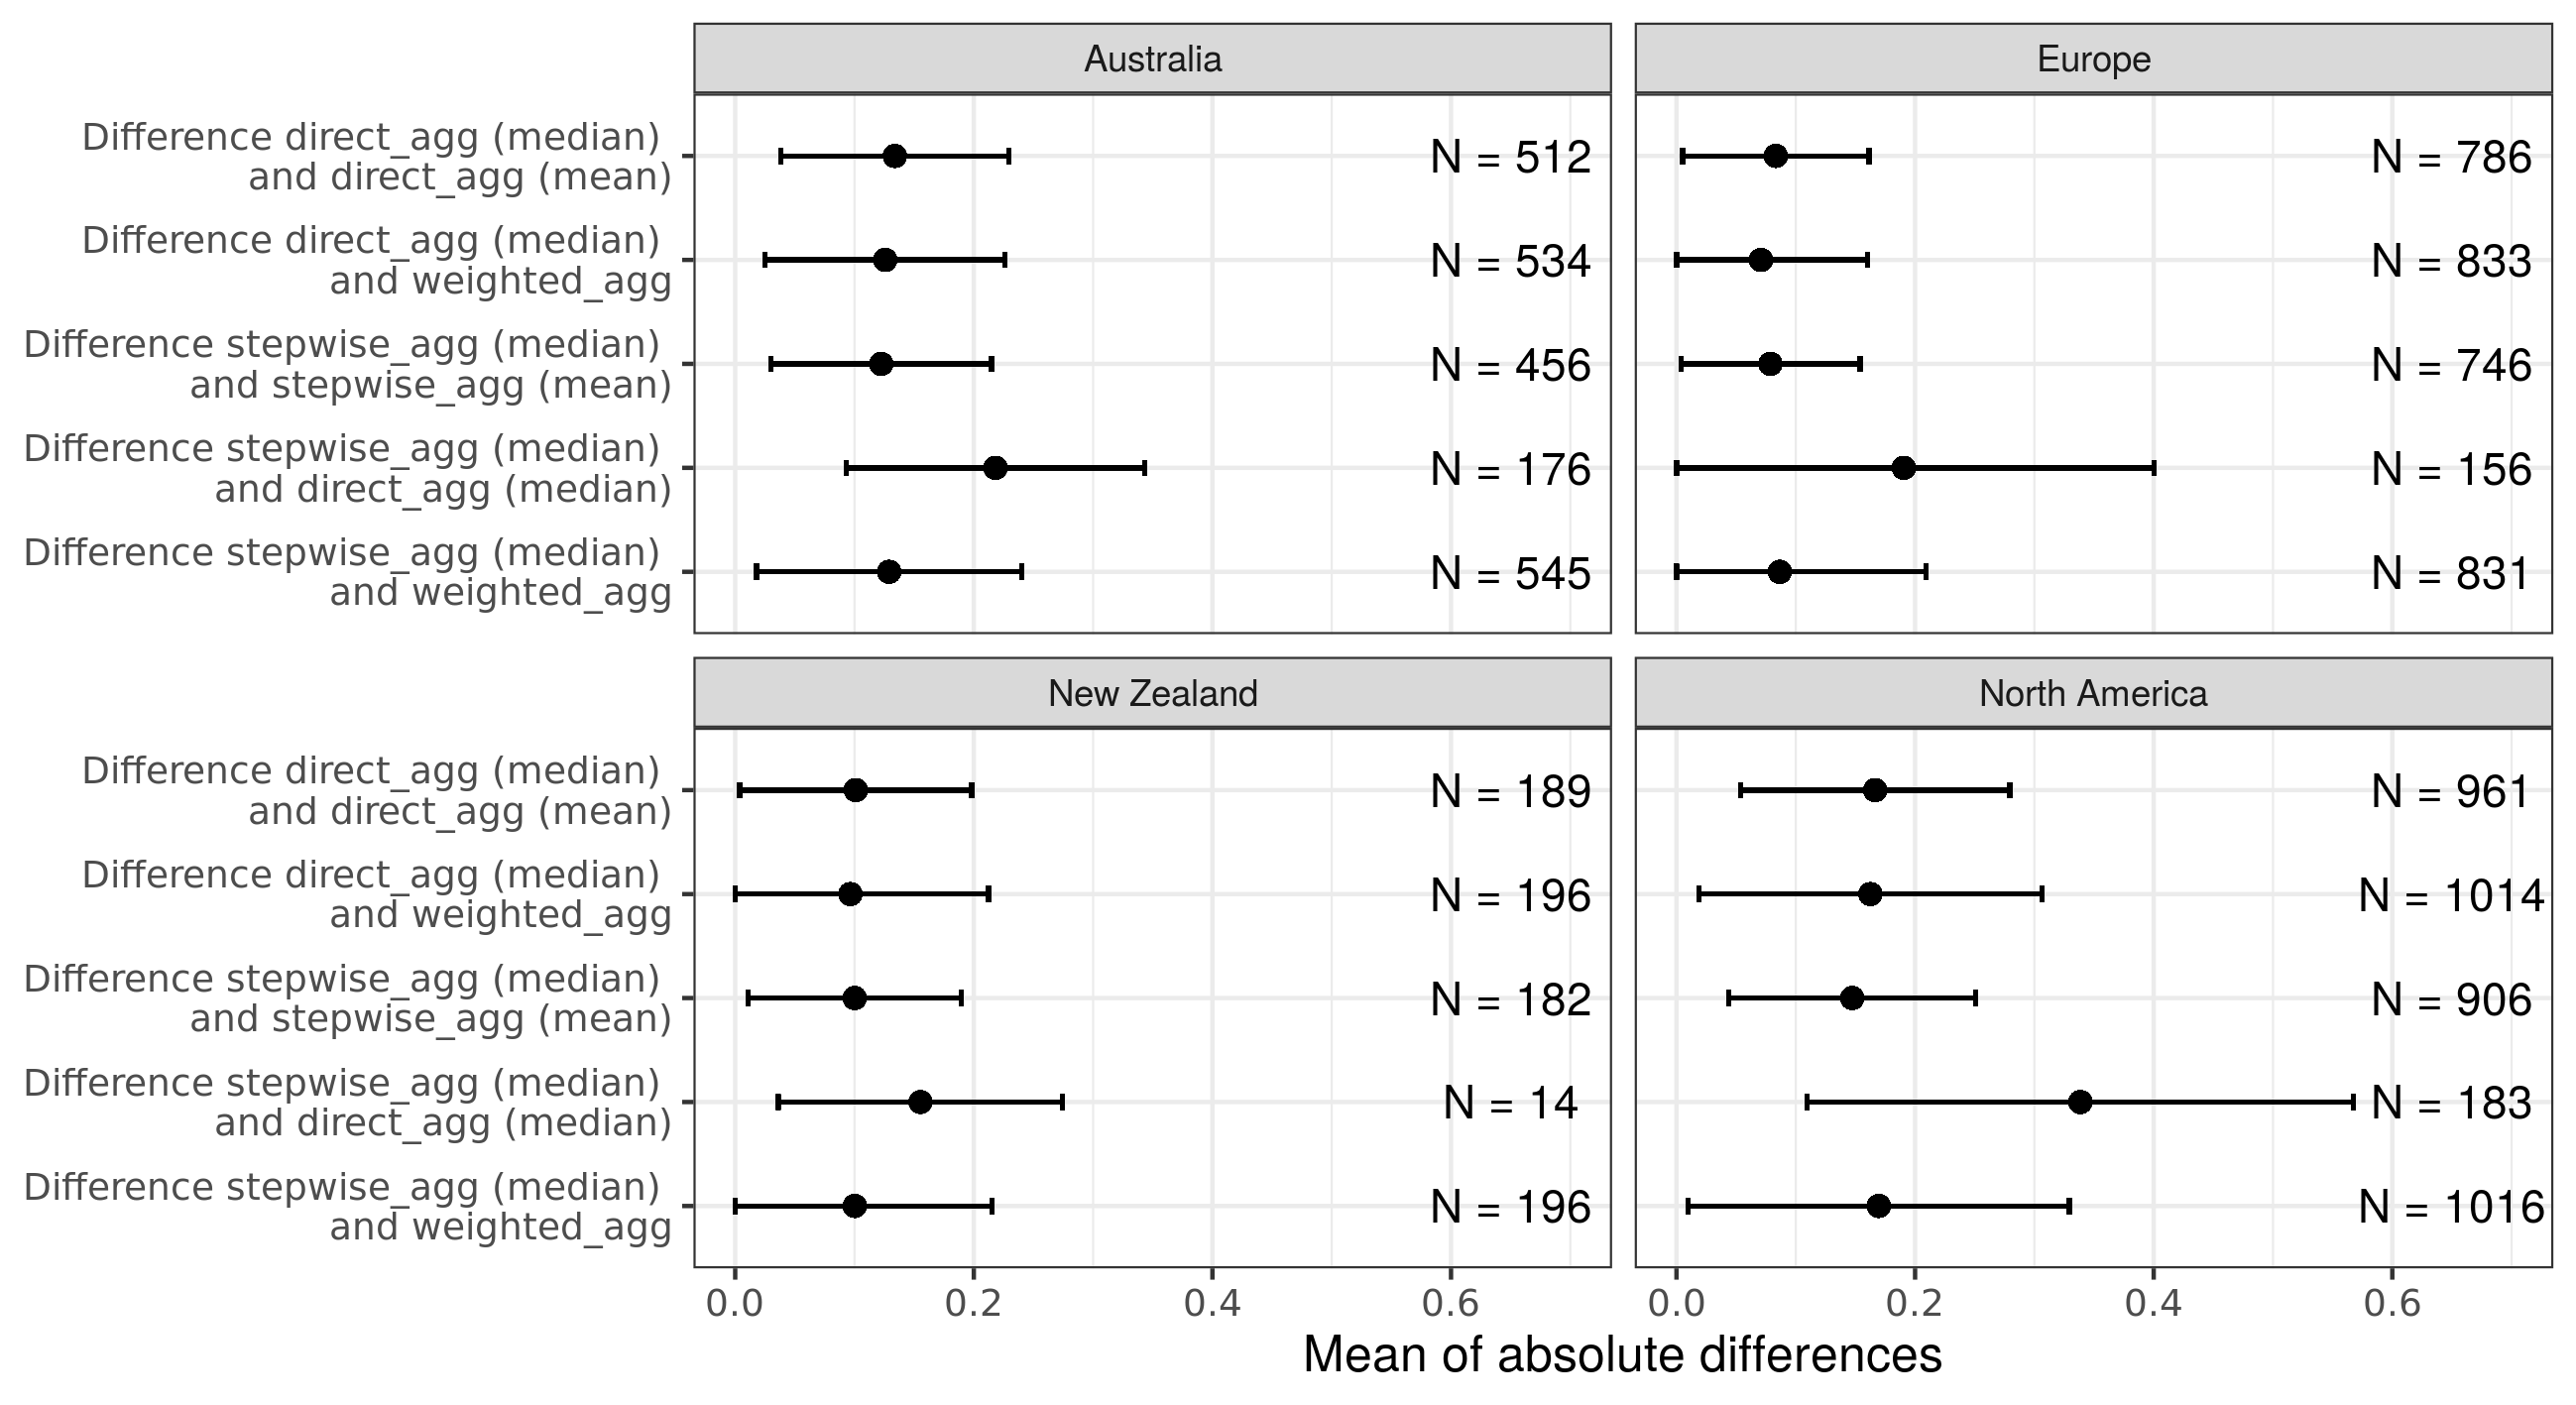
\includegraphics[width=16.5cm, height=10cm]{Comparison_trait_agg_methods.png}
%     \caption{Comparison of trait aggregation methods when aggregating over all traits for all datasets. Displayed are means of absolute differences in trait affinities with standard deviations (truncated at 0). Compared aggregation methods are displayed on the y-axis. N indicates the number of cases where differences occurred. Total number of cases: Australia 2223, Europe 3352, New Zealand 777, and North America 4080.}
%     \label{fig:comp_aggr_methods}
% \end{figure}

%\subsubsection*{Simulation of varying taxonomic hierarchies}
 
% \begin{figure}[H]
%     \centering
%     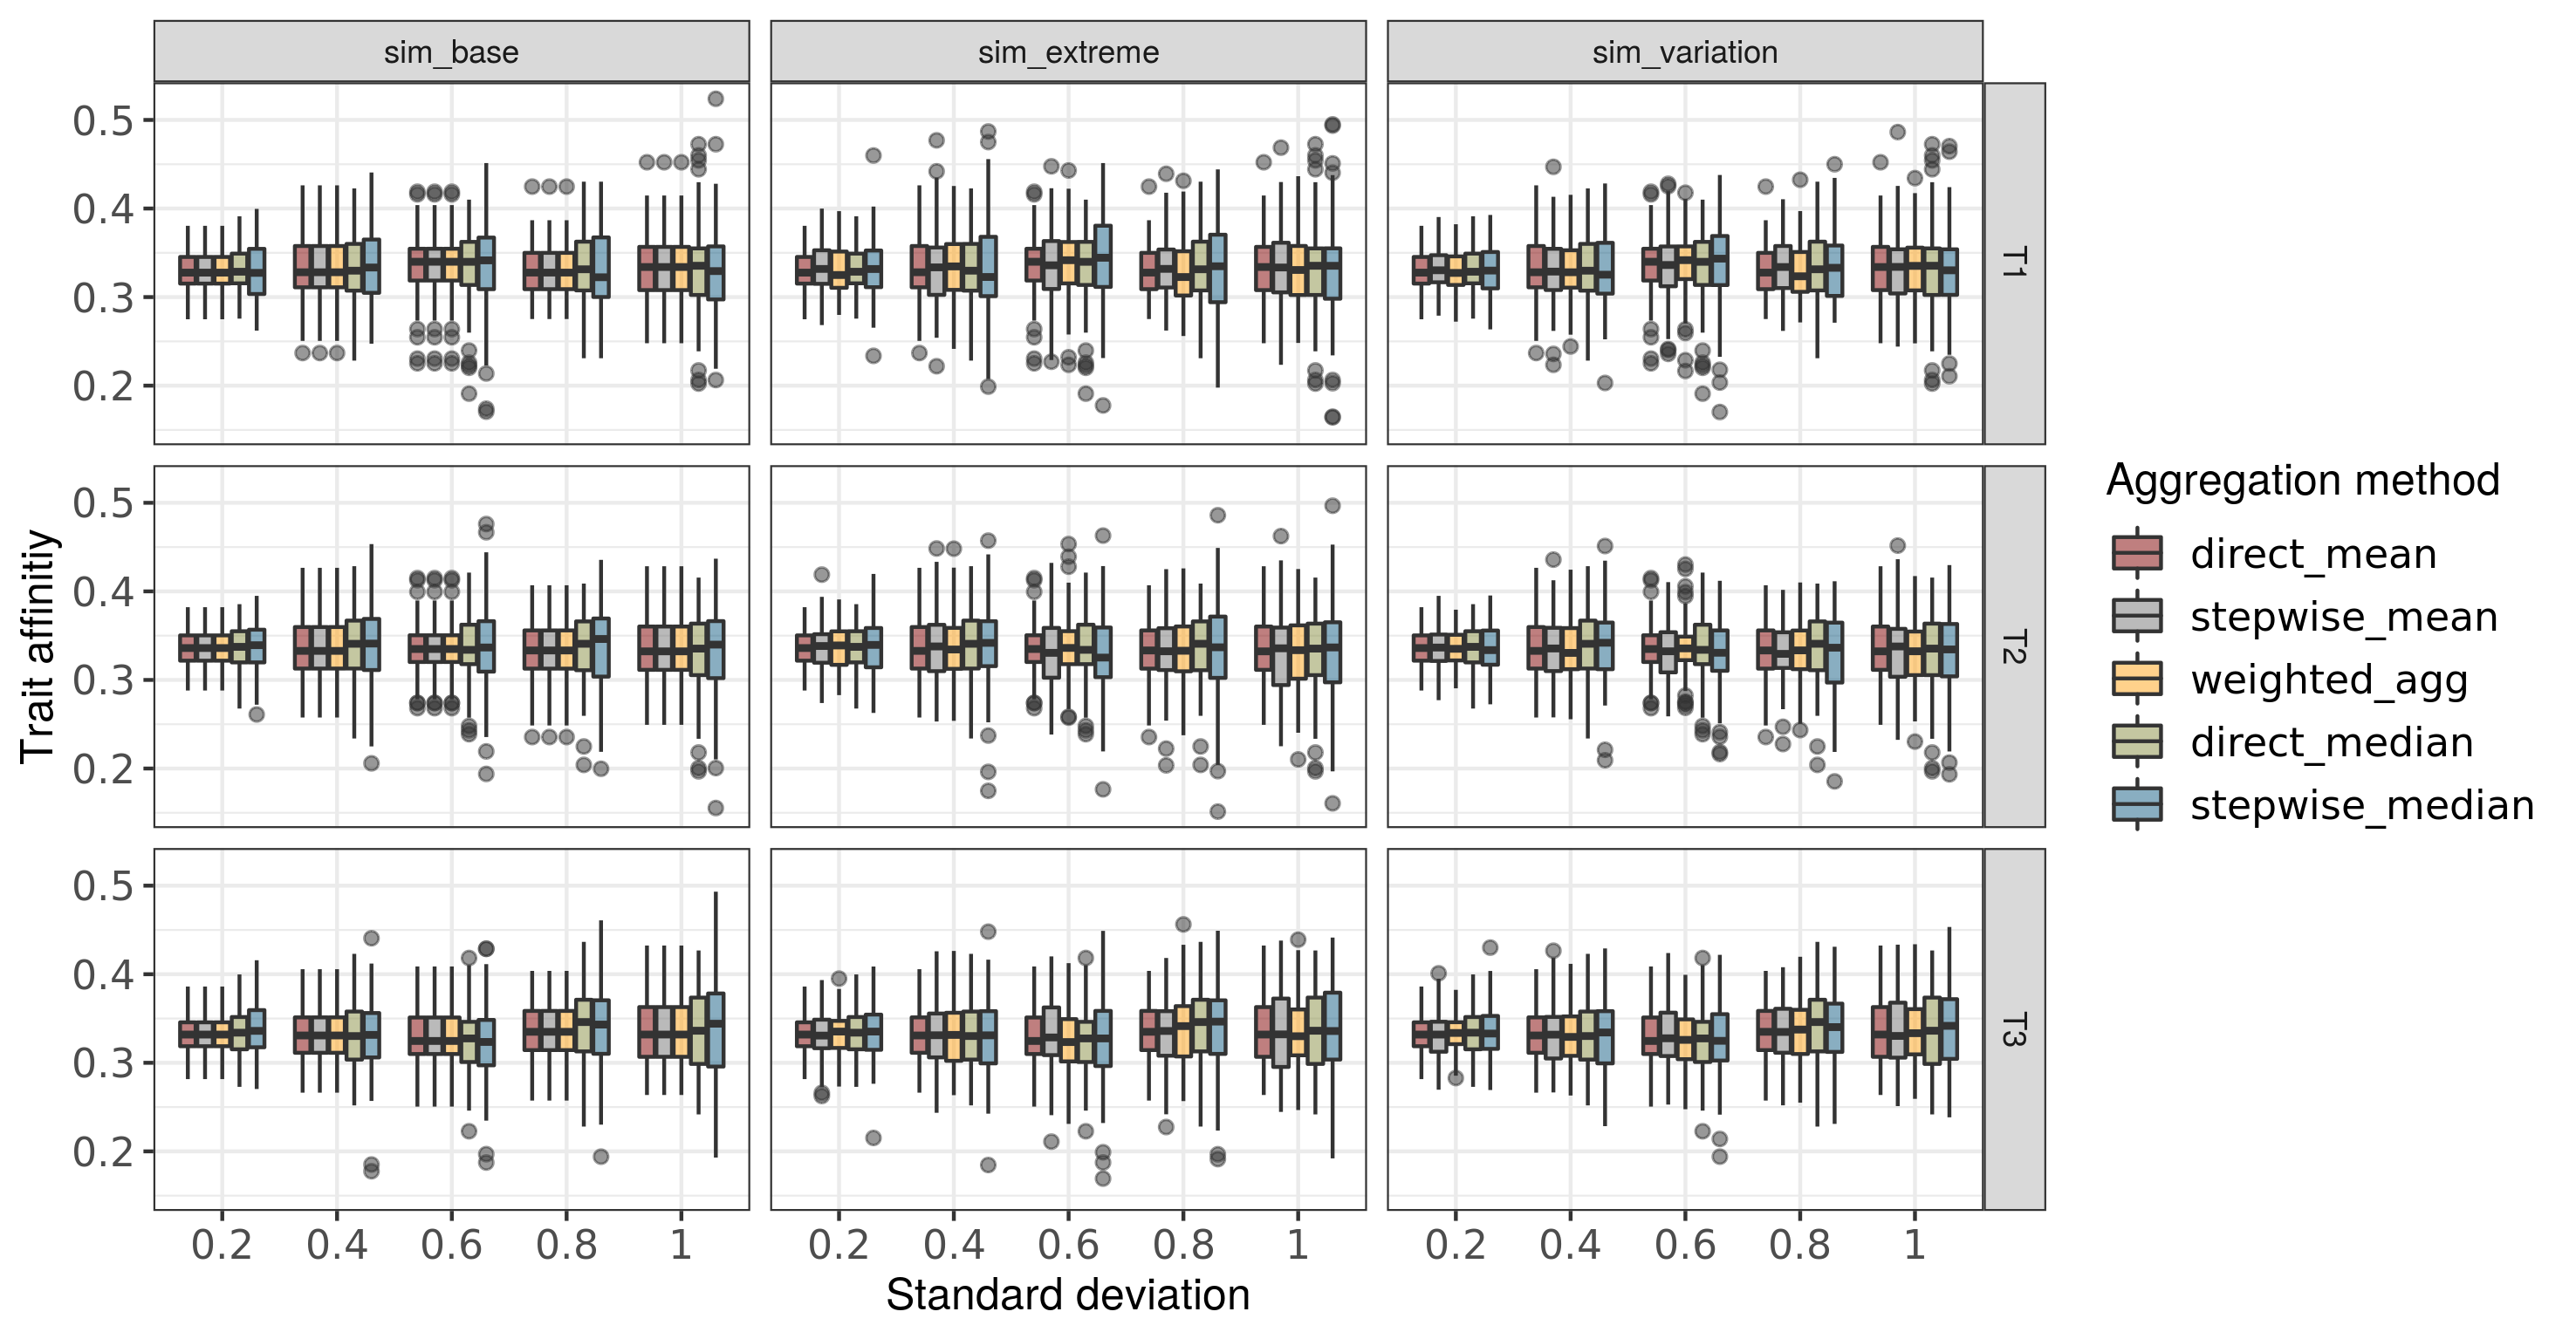
\includegraphics[width=16.5cm, height=10cm]{Overview_sim_results.png}
%     \caption{Ranges of aggregated trait affinities for the three examples of taxonomic hierarchies and simulated levels of trait variability. Boxplots depict results for each trait aggregation method of 100 simulations. T1 to T3 are the simulated traits.}
%     \label{fig:overview_sim_results}
% \end{figure}

% \begin{figure}[H]
%     \centering
%     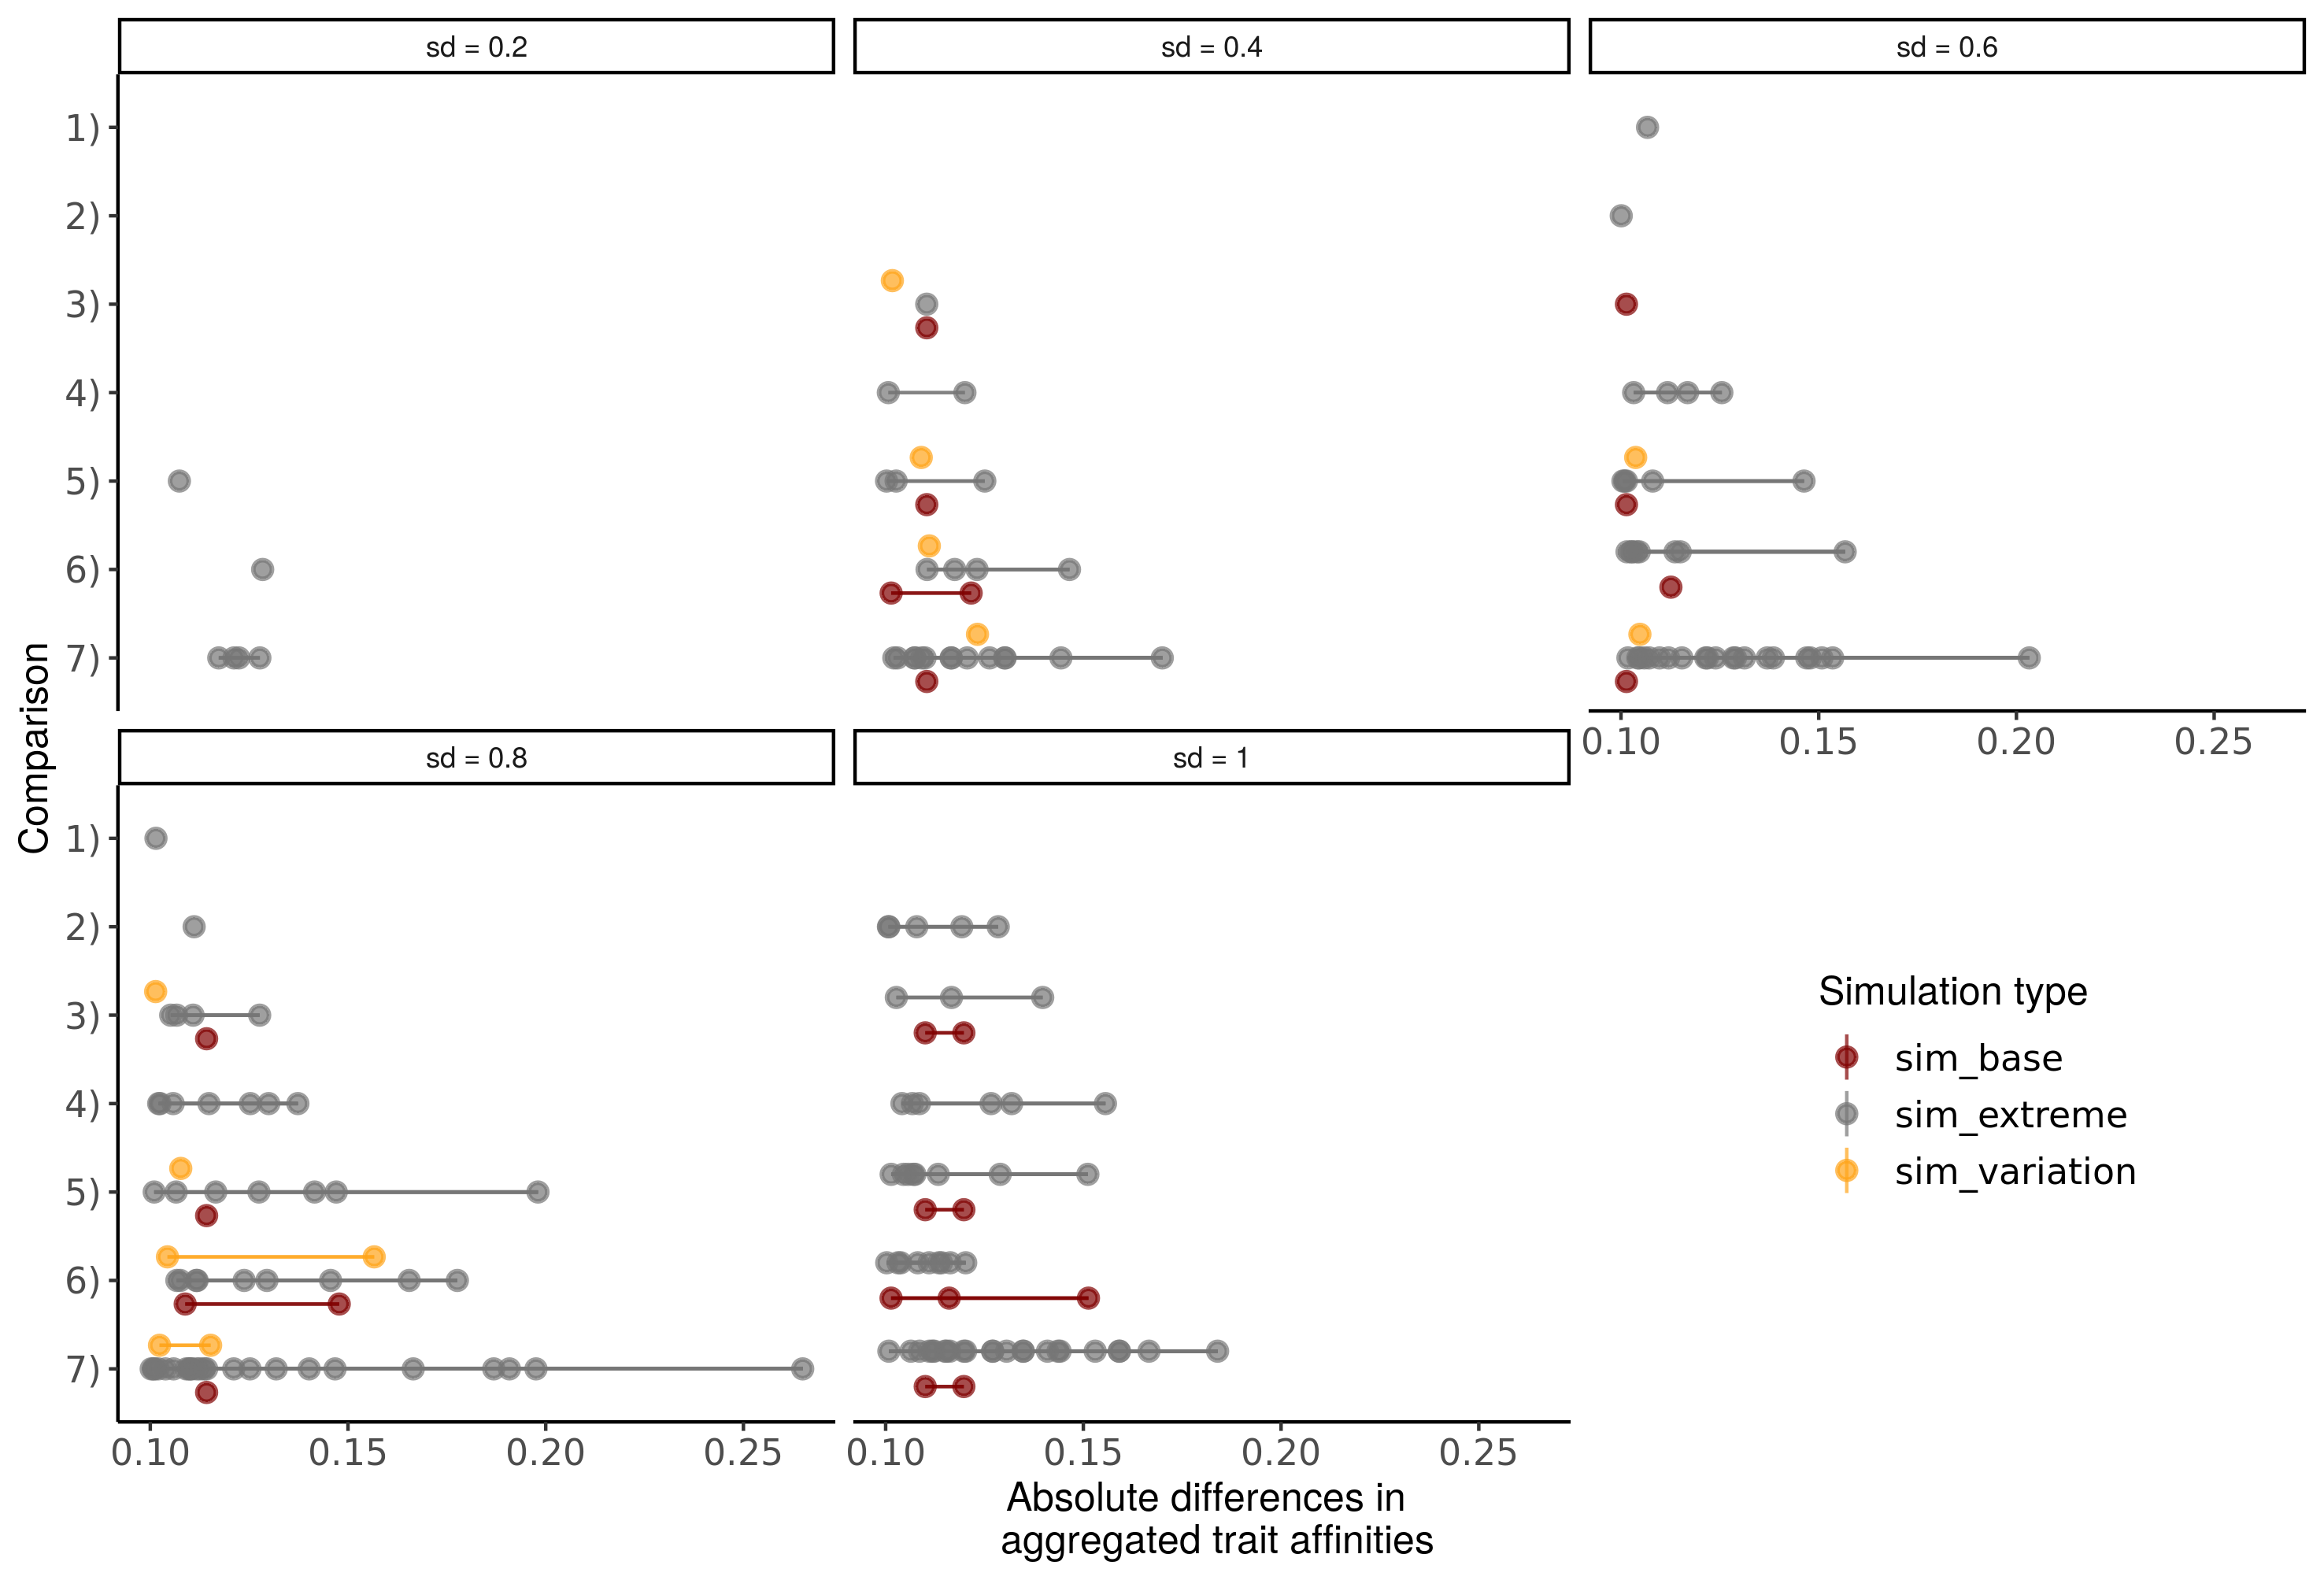
\includegraphics[width=16.5cm, height=10cm]{Diffs_indiv_runs_sim.png}
%     \caption{Comparison of the results of the trait aggregation methods for every simulated dataset. Simulated datasets where absolute differences between aggregated trait affinities were greater than 0.1 are depicted. Only the comparisons are shown were differences greater than 0.1 occurred.}
%     \label{fig:sim_indv_runs}
% \end{figure}

\subsubsection*{Taxonomic hierarchy in the trait datasets used for comparisons with assigned traits at family level}
\label{sec:taxonomic_hierarchy}
% \begin{figure}[H]
%     \centering
%     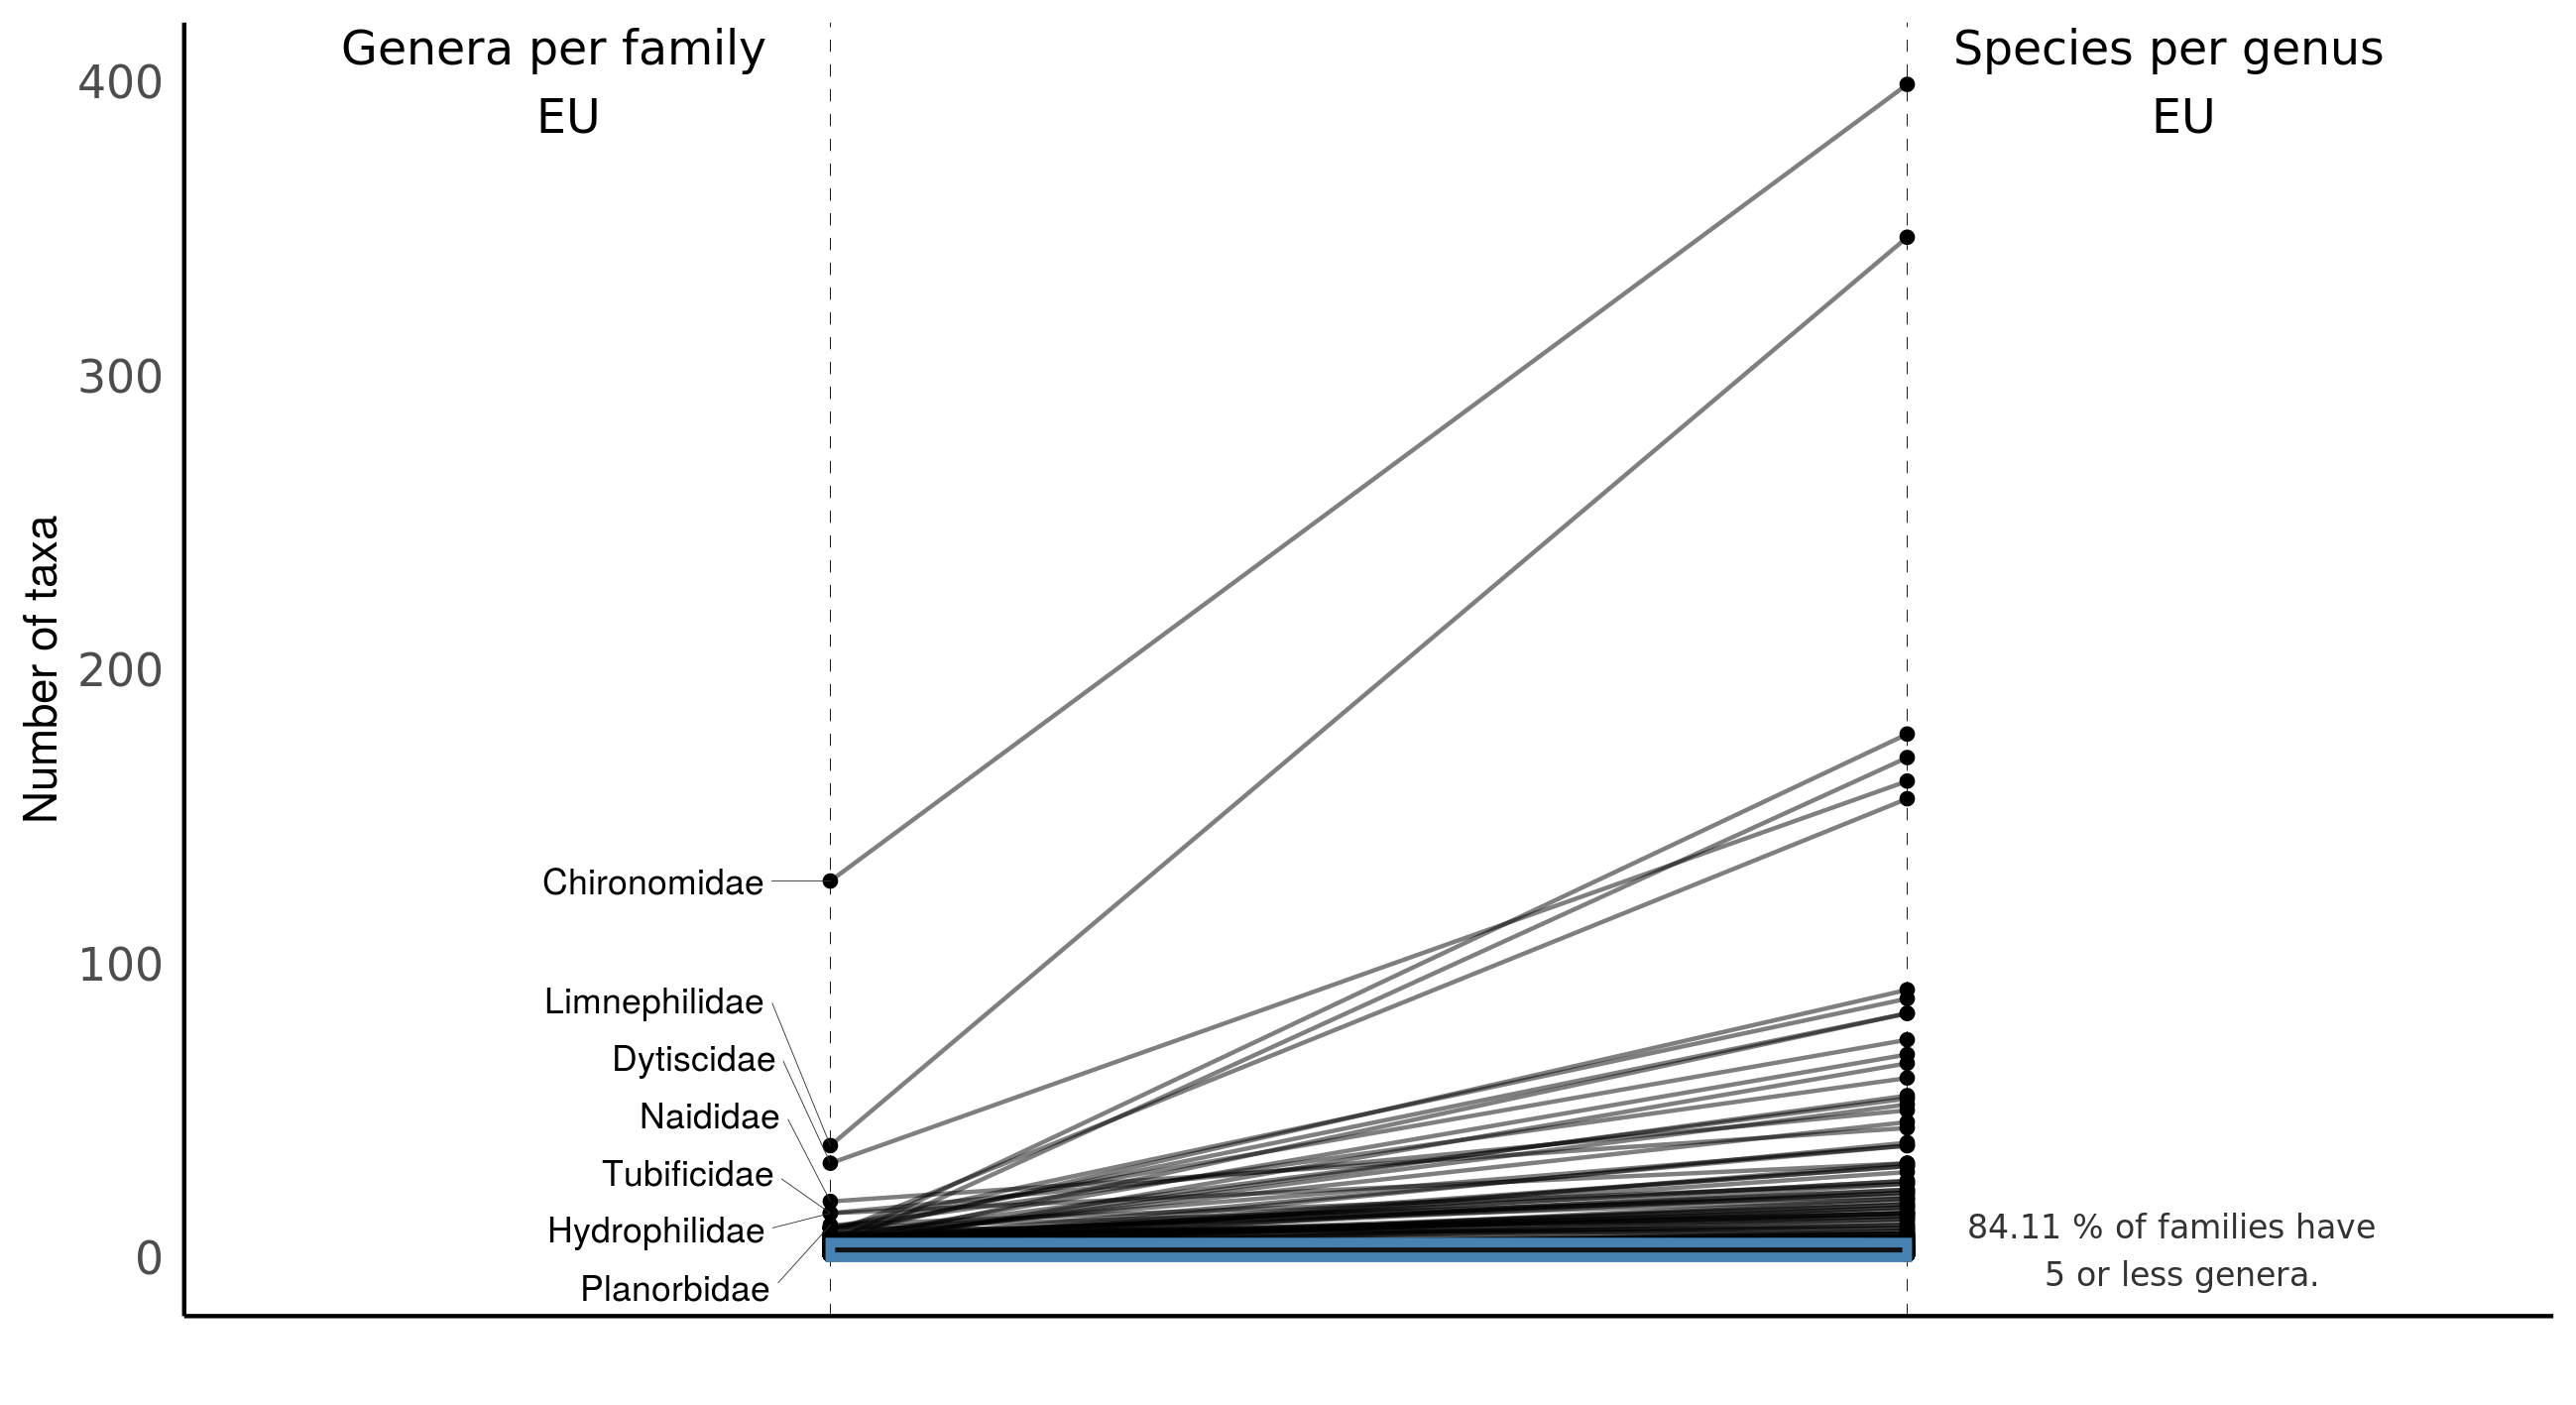
\includegraphics[width=16.5cm, height=10cm]{taxonomic_hierarchy_EU.png}
%     \caption{Number of genera per family and species per genus for the European trait dataset. For better visual display only families with more than 10 genera are displayed.}
%     \label{fig:tax_hierarchy_EU}
% \end{figure}

\begin{figure}[H]
    \centering
    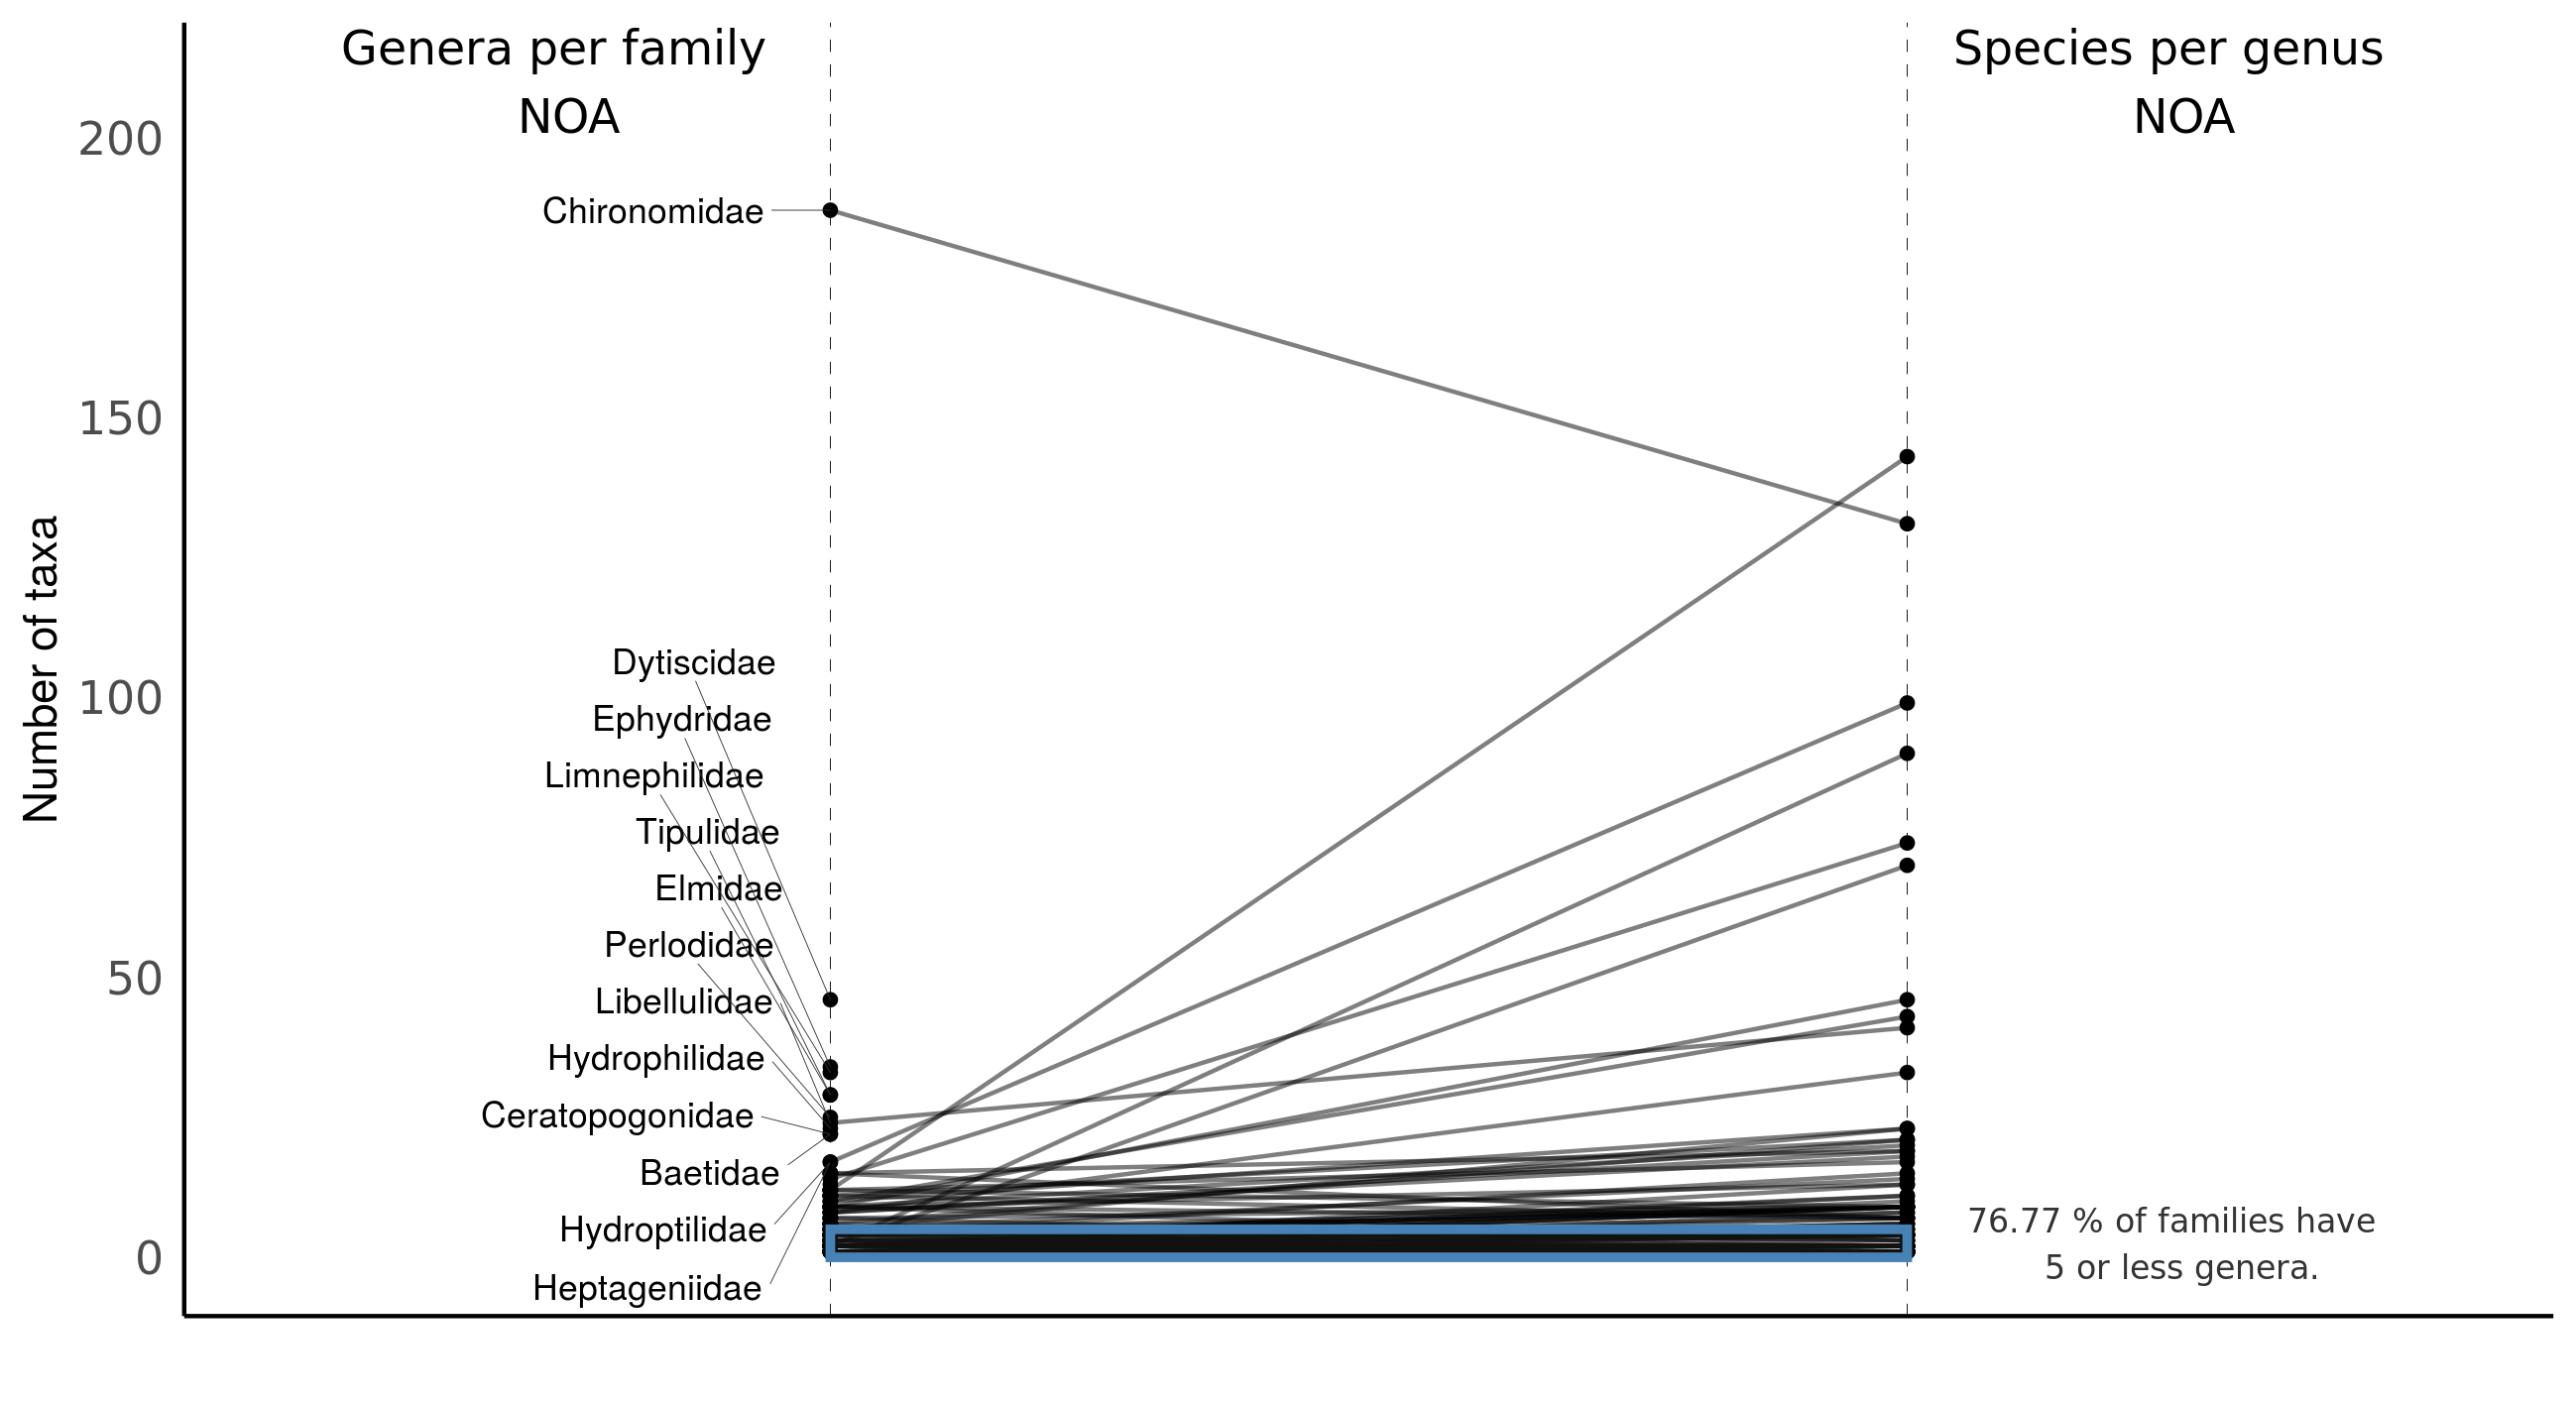
\includegraphics[width=16.5cm, height=10cm]{taxonomic_hierarchy_NOA.png}
    \caption{Number of genera per family and species per genus for those families of the North American trait dataset that have been compared with assigned traits at family level. For better visual display only families with more than 15 genera are displayed.}
    \label{fig:tax_hierarchy_NOA}
\end{figure}

\begin{figure}[H]
    \centering
    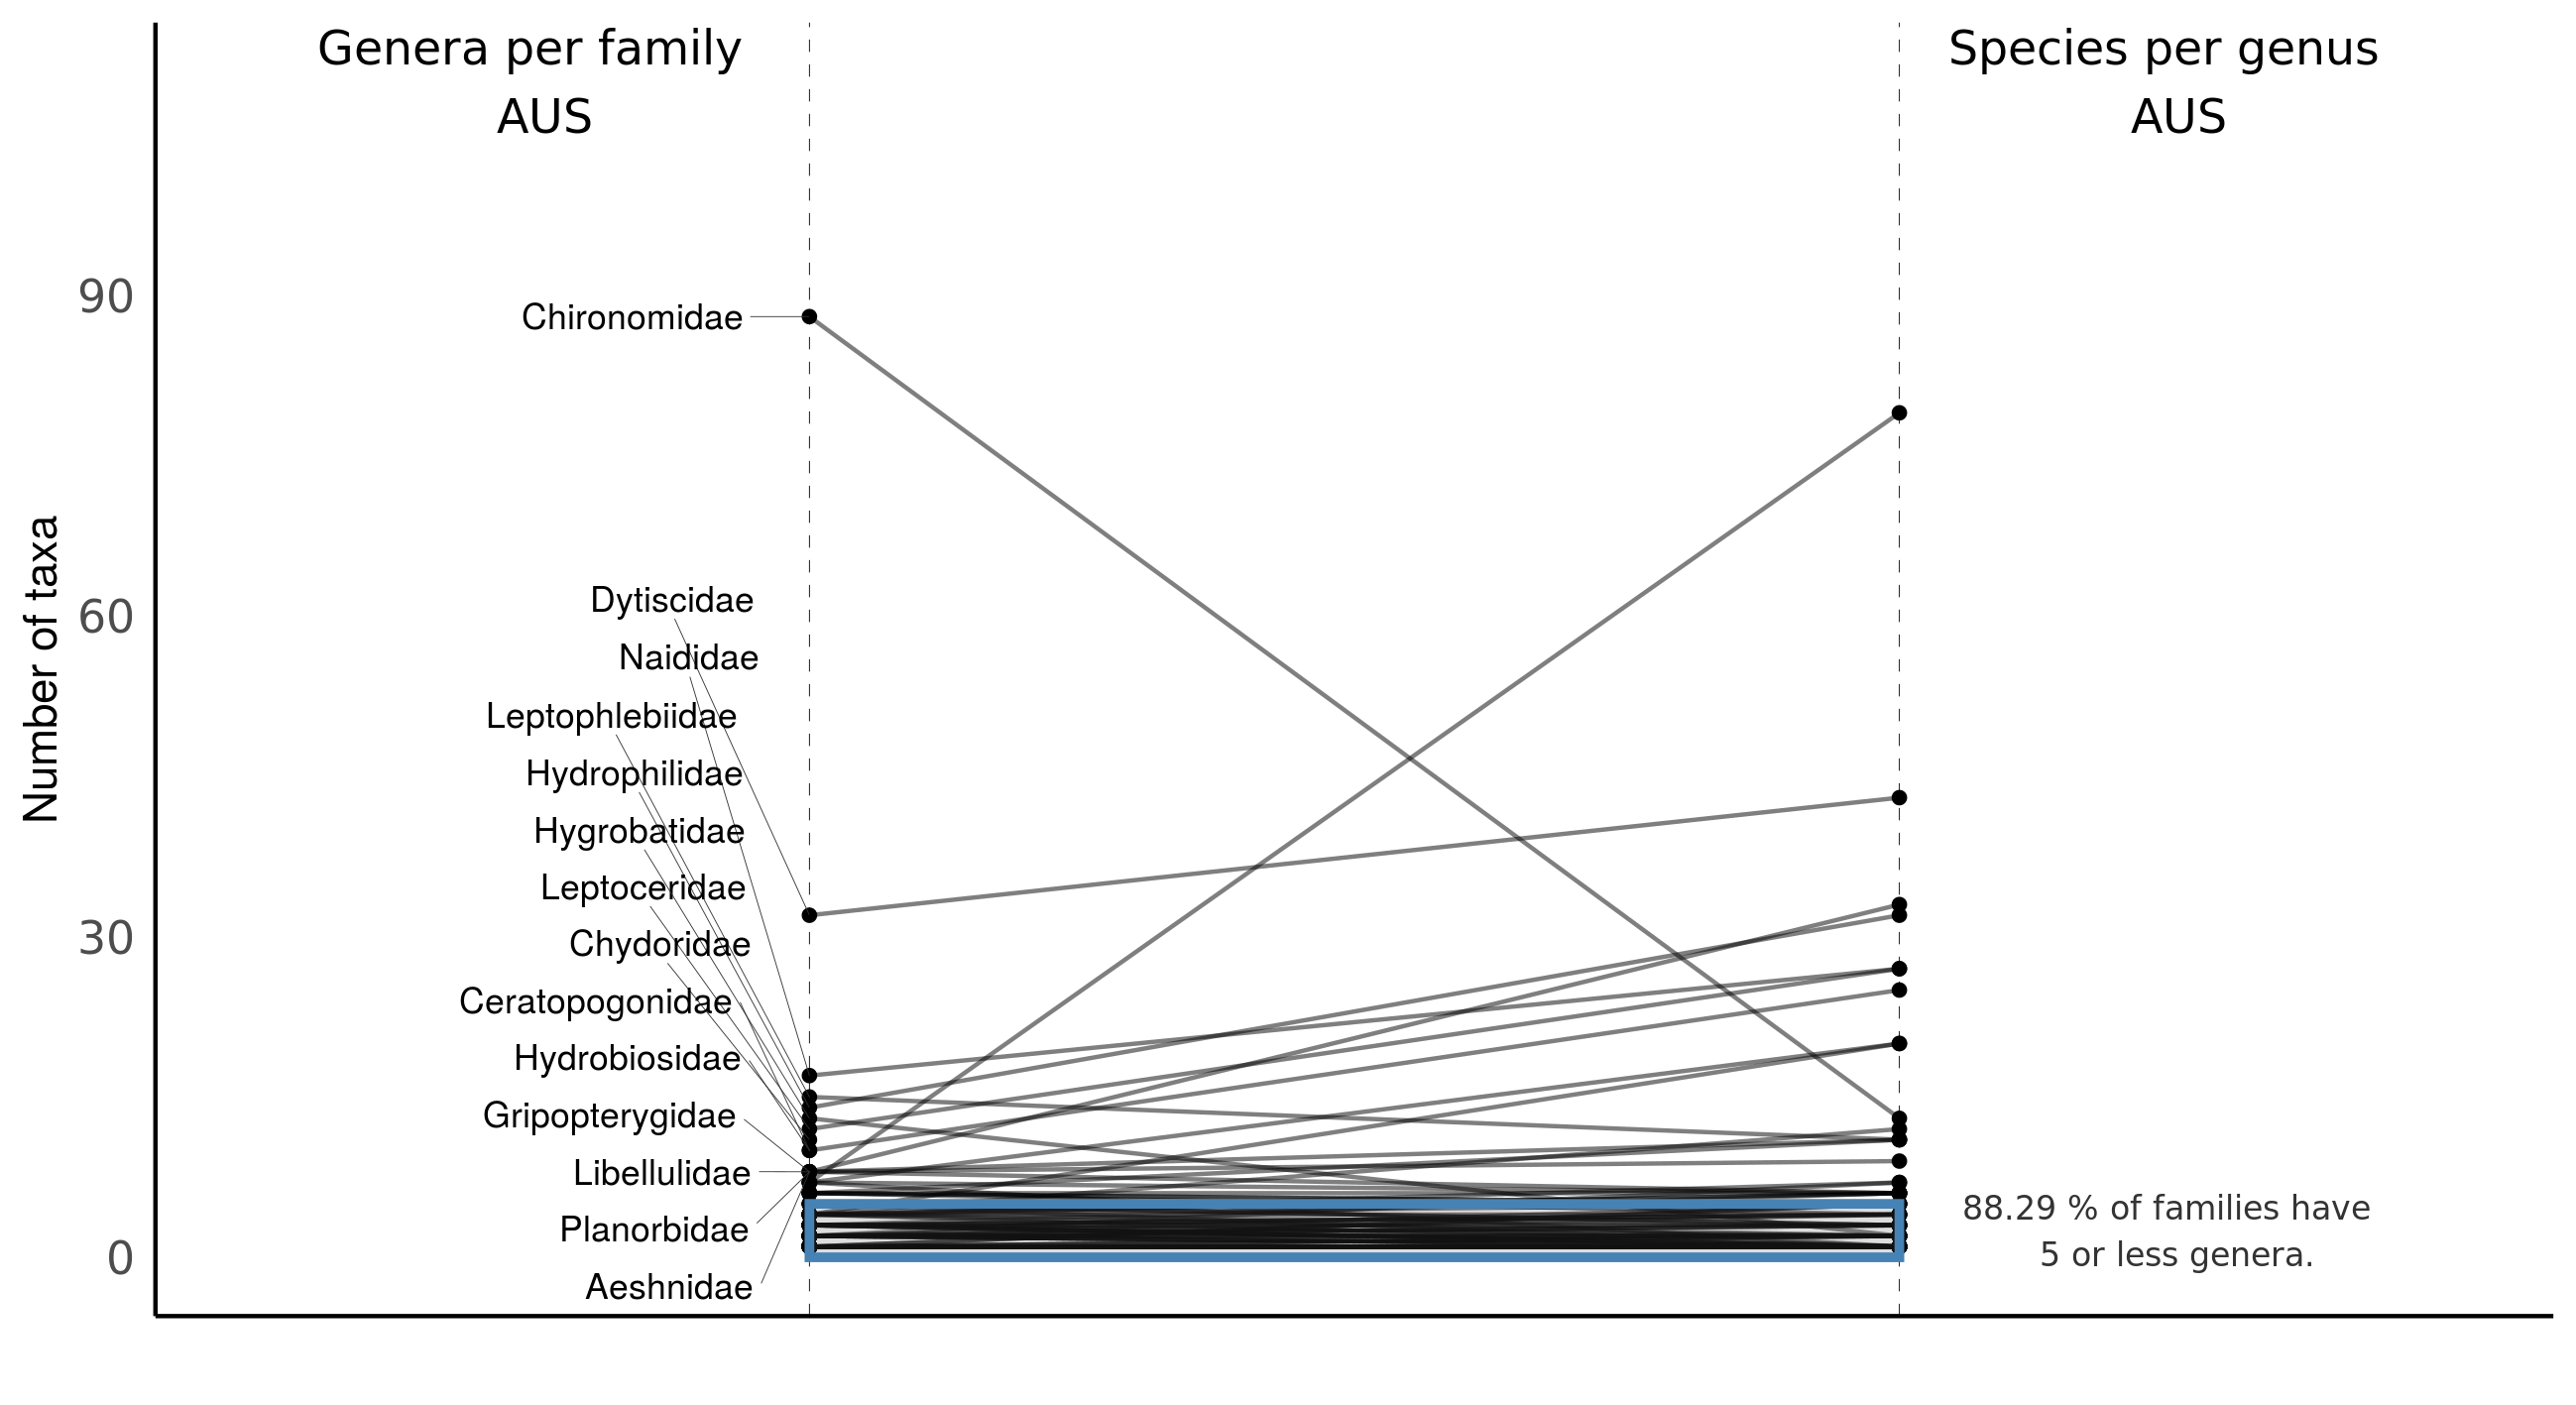
\includegraphics[width=16.5cm, height=10cm]{taxonomic_hierarchy_AUS.png}
    \caption{Number of genera per family and species per genus for the Australian trait dataset. For better visual display only families with more than 7 genera are displayed.}
    \label{fig:tax_hierarchy_AUS}
\end{figure}

% \begin{figure}[H]
%     \centering
%     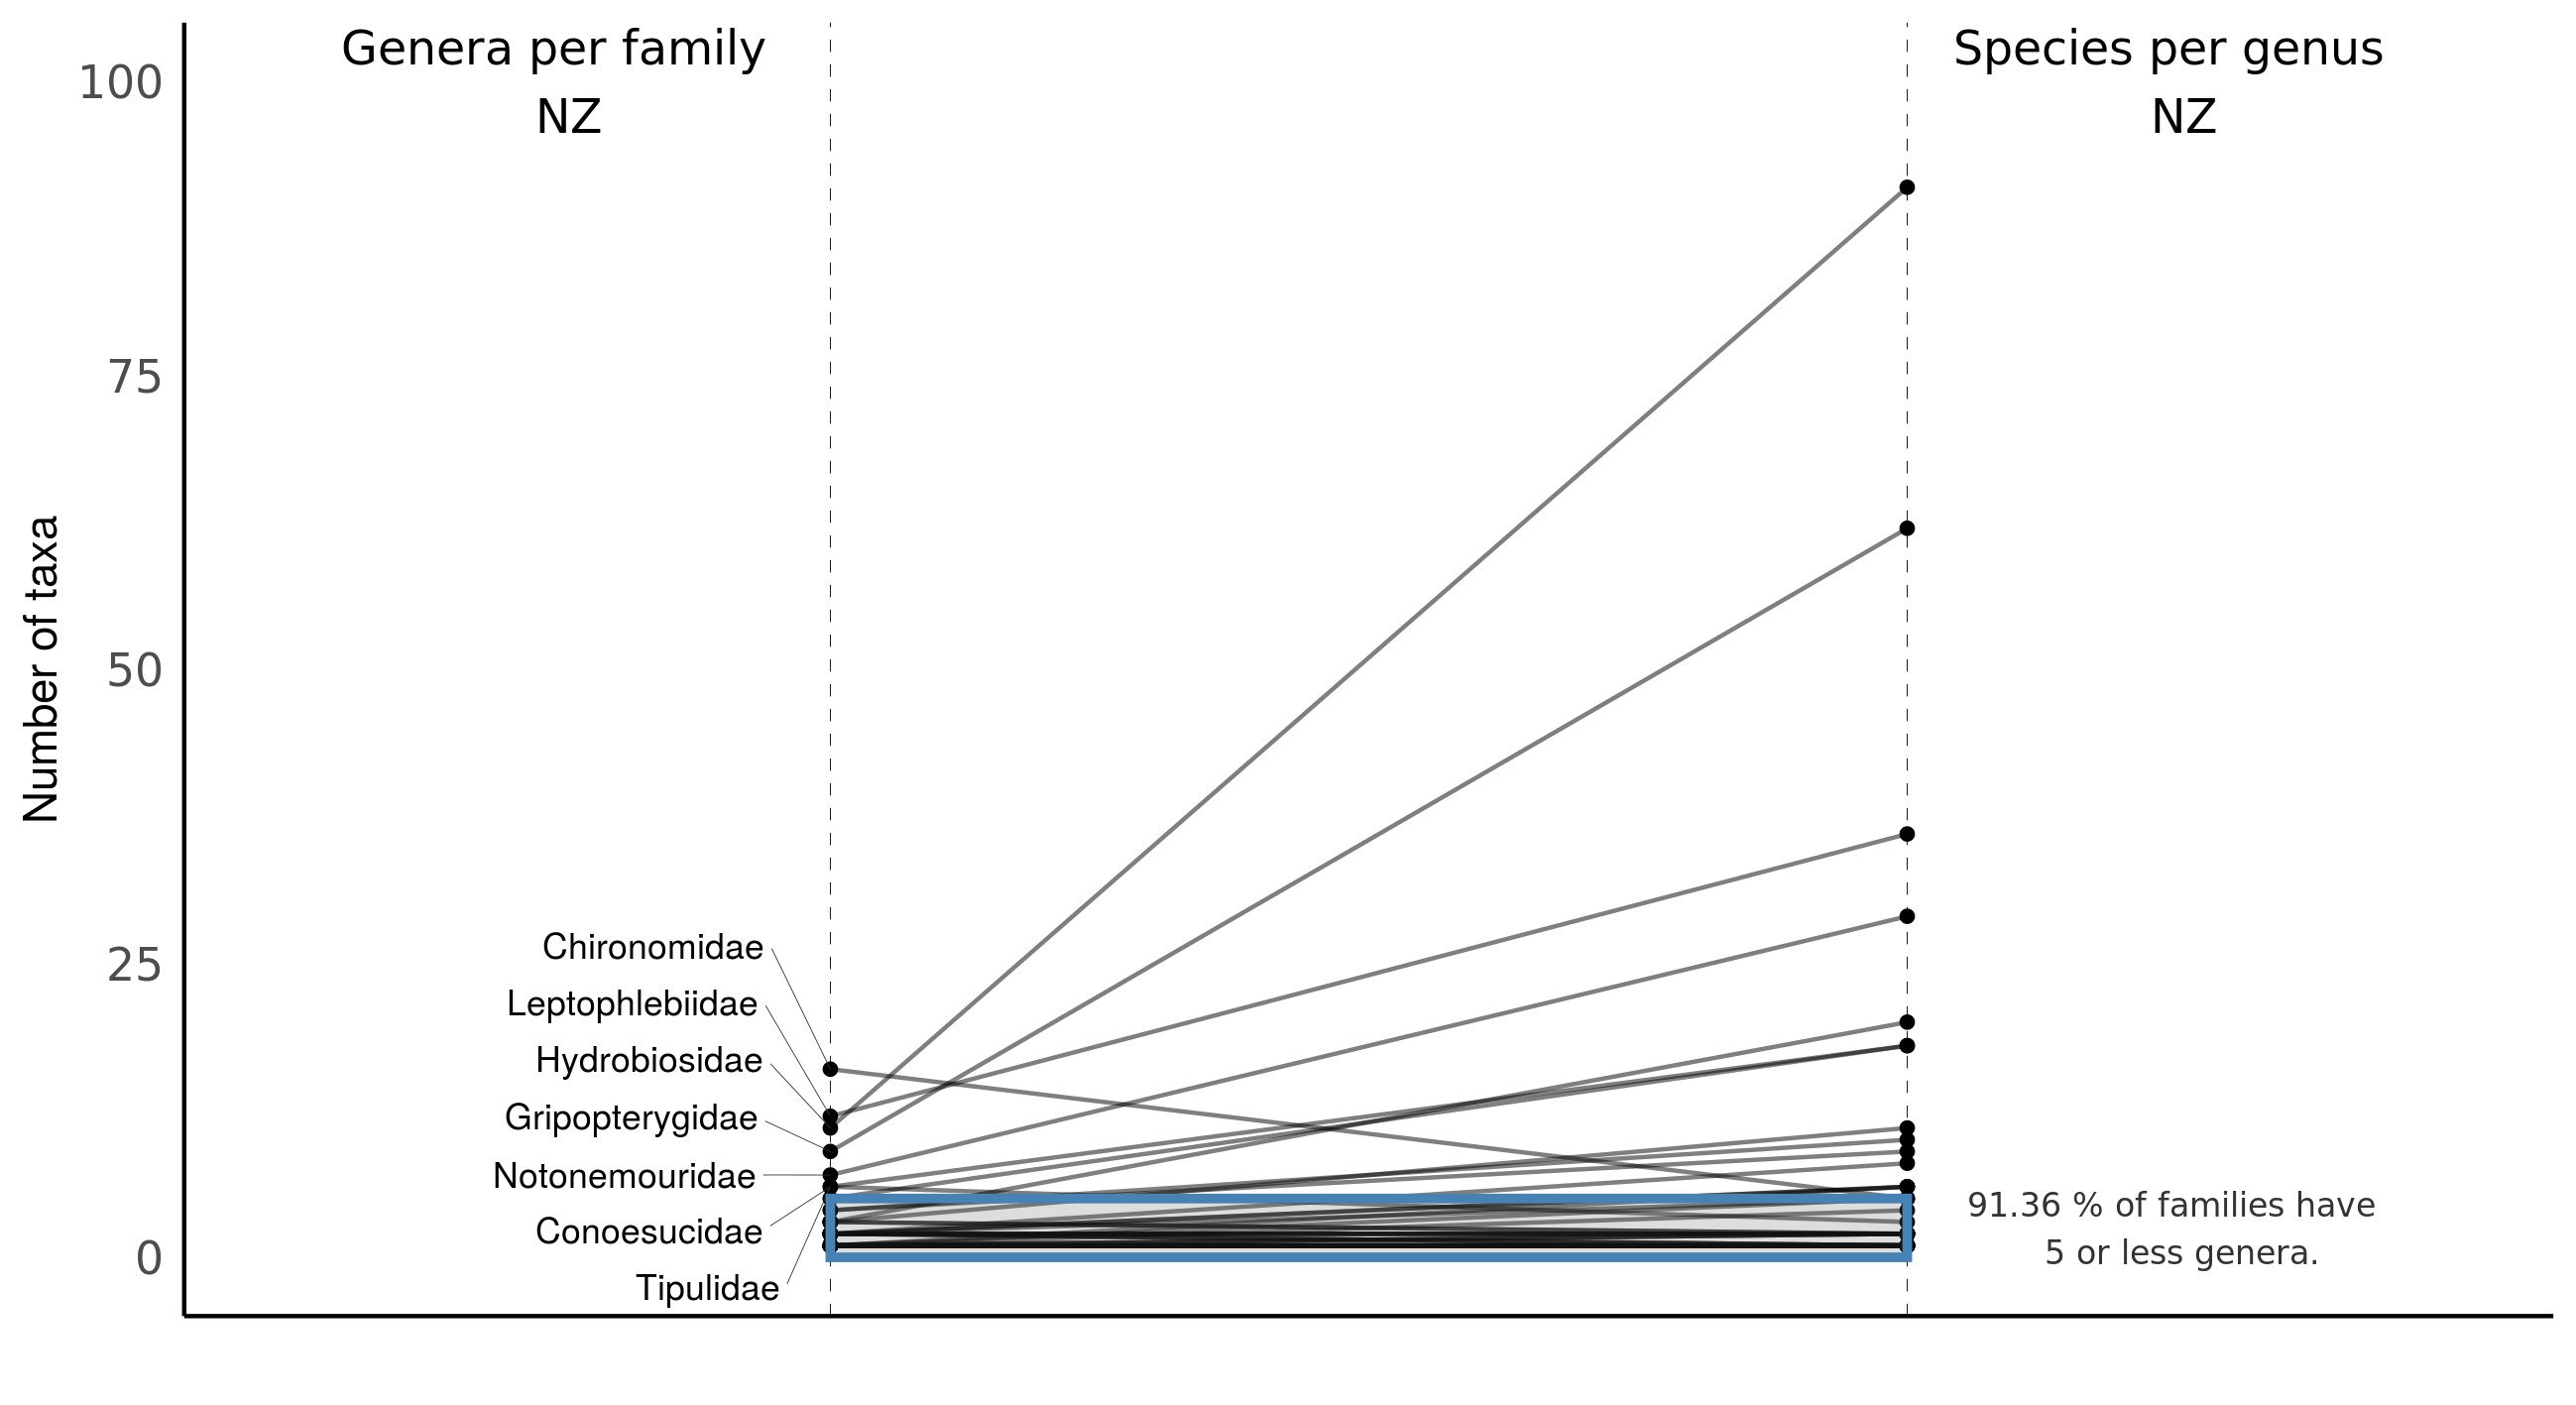
\includegraphics[width=16.5cm, height=10cm]{taxonomic_hierarchy_NZ.png}
%     \caption{Number of genera per family and species per genus for the New Zealand trait dataset. For better visual display only families with more than 5 genera are displayed.}
%     \label{fig:tax_hierarchy_NZ}
% \end{figure}

\newpage

\subsection*{Re-analysis of Szöcs et al. using harmonised and aggregated grouping features}

\begin{table}[ht]
    \centering
    \caption{Mean, median and standard deviation of the affinities of traits that were responsive to the salinity gradient in the original study but not in the re-analysis using the harmonised European trait dataset.} 
    \label{tab:SI_resp_traits_summary_stats}
    \begin{tabular}{llccc|c}
    \toprule[.1em]
    Type & Trait & Mean & Median & SD & Responsive? \\ 
    \toprule[.1em]
    Stepw\_median & Shredder & 0.20 & 0.14 & 0.25 & No \\ 
      Stepw\_mean & Shredder & 0.18 & 0.12 & 0.22 & No\\ 
      Direct\_median & Shredder & 0.21 & 0.14 & 0.25 & No\\ 
      Direct\_mean & Shredder & 0.19 & 0.14 & 0.22 & No\\ 
      Weighted & Shredder & 0.19 & 0.14 & 0.22 & No \\ 
      Harmonised; not\_aggregated & Shredder & 0.18 & 0.12 & 0.24 & No \\ 
      Original & Shredder & 0.25 & 0.14 & 0.32 & Yes\\ 
      \midrule
      Stepw\_median & Gills & 0.30 & 0.27 & 0.32 & Yes\\ 
      Stepw\_mean & Gills & 0.29 & 0.22 & 0.32 & Yes\\ 
      Direct\_median & Gills & 0.30 & 0.30 & 0.32 & Yes\\ 
      Direct\_mean & Gills & 0.30 & 0.30 & 0.32 & Yes\\ 
      Weighted & Gills & 0.30 & 0.30 & 0.32 & Yes\\ 
      Harmonised; not\_aggregated & Gills & 0.30 & 0.25 & 0.32 & No \\ 
      Original & Gills & 0.28 & 0.00 & 0.33 & Yes \\ 
      \midrule
      Stepw\_median & Short life cycle & 0.64 & 0.75 & 0.39 & No \\ 
      Stepw\_mean & Short life cycle & 0.64 & 0.79 & 0.39 & No \\ 
      Direct\_median & Short life cycle & 0.67 & 0.75 & 0.37 & Yes \\ 
      Direct\_mean & Short life cycle & 0.67 & 0.79 & 0.38 & Yes \\ 
      Weighted & Short life cycle & 0.67 & 0.79 & 0.38 & Yes\\ 
      Harmonised; not\_aggregated & Short life cycle & 0.64 & 0.75 & 0.40 & Yes \\ 
      Original & Short life cycle & 0.64 & 0.75 & 0.40 & Yes \\ 
      \midrule
      Stepw\_median & Long life cylce & 0.36 & 0.25 & 0.39 & No \\ 
      Stepw\_mean & Long life cylce & 0.36 & 0.21 & 0.39 & No \\
      Direct\_median & Long life cylce & 0.33 & 0.25 & 0.37 & Yes\\ 
      Direct\_mean & Long life cylce & 0.33 & 0.21 & 0.38 & Yes \\ 
      Weighted & Long life cylce & 0.33 & 0.21 & 0.38 & Yes \\ 
      Harmonised; not\_aggregated & Long life cylce & 0.36 & 0.25 & 0.40 & Yes \\ 
      Original & Long life cylce & 0.36 & 0.25 & 0.40 & Yes\\ 
    \bottomrule
    \end{tabular}
\end{table}

%\subsection*{Re-analysis of Szöcs et al. using harmonized grouping features.}
%\label{subsec:SI_szoecs_reanalysis}

% \subsubsection*{RDA of trait composition}

% \begin{figure}[H]
%     \centering
%     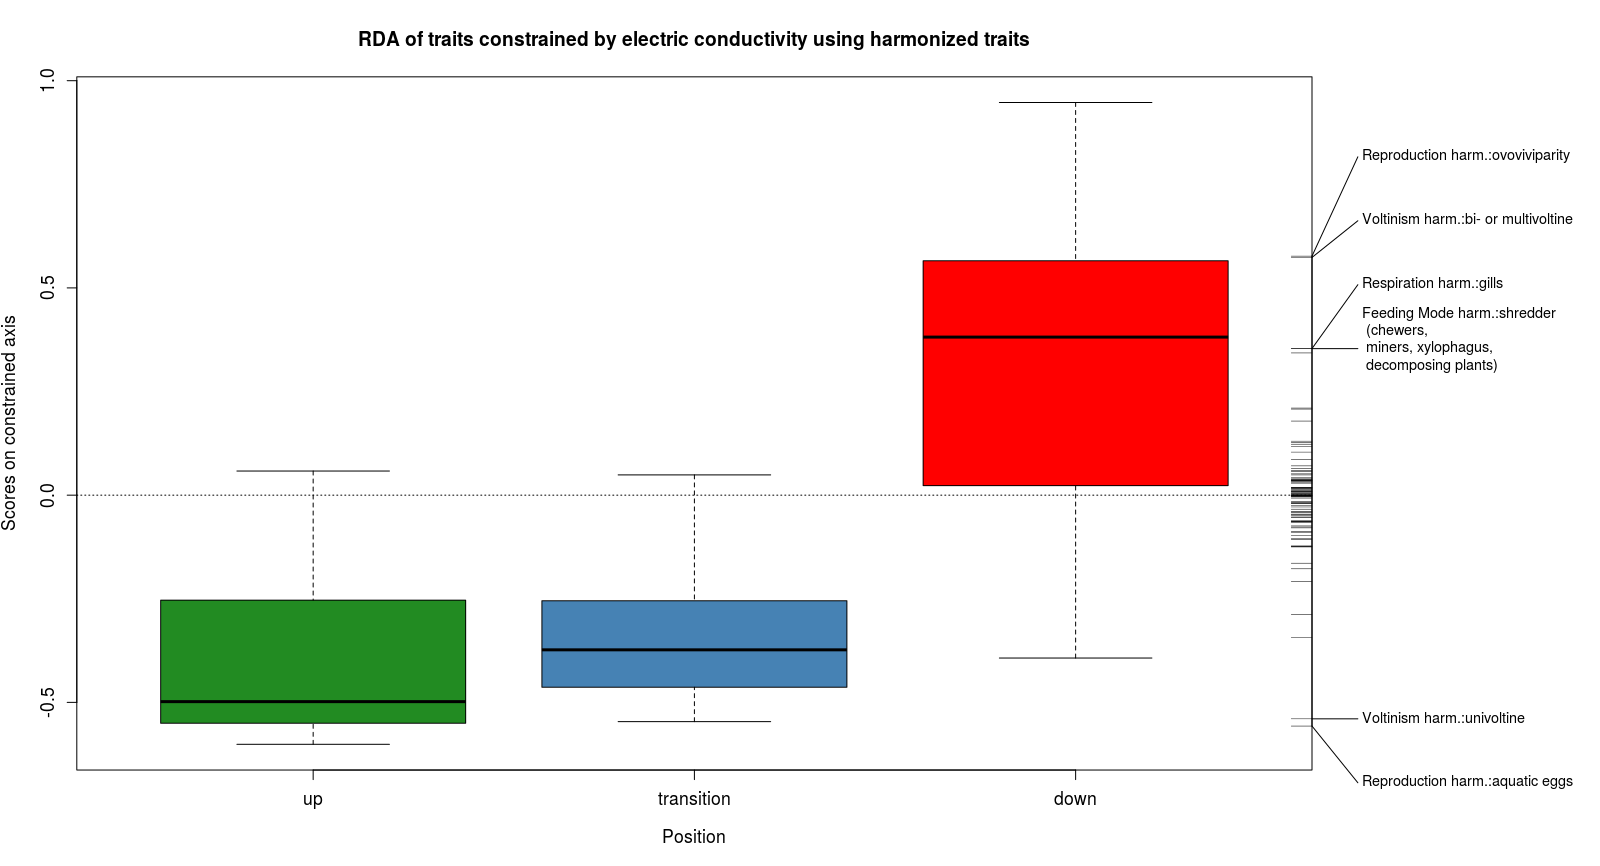
\includegraphics[width=16.5cm, height=10cm]{RDA_traits_harmonized.png}
%     \caption{RDA of traits constrained by electric conductivity using harmonized grouping features. Boxplot of site scores along the conductivity axis ($31.44 \%$ explained variance, p = 0.001, 1000 permutations). Rug on the right indicates trait scores on the conductivity axis. Only traits with a mahalanobis distance greater than 5.02 were labeled in accordance to the procedure in Szöcs et al. \cite{szocs_effects_2014}.
%     } 
% \end{figure}

% \begin{figure}[H]
%     \centering
%     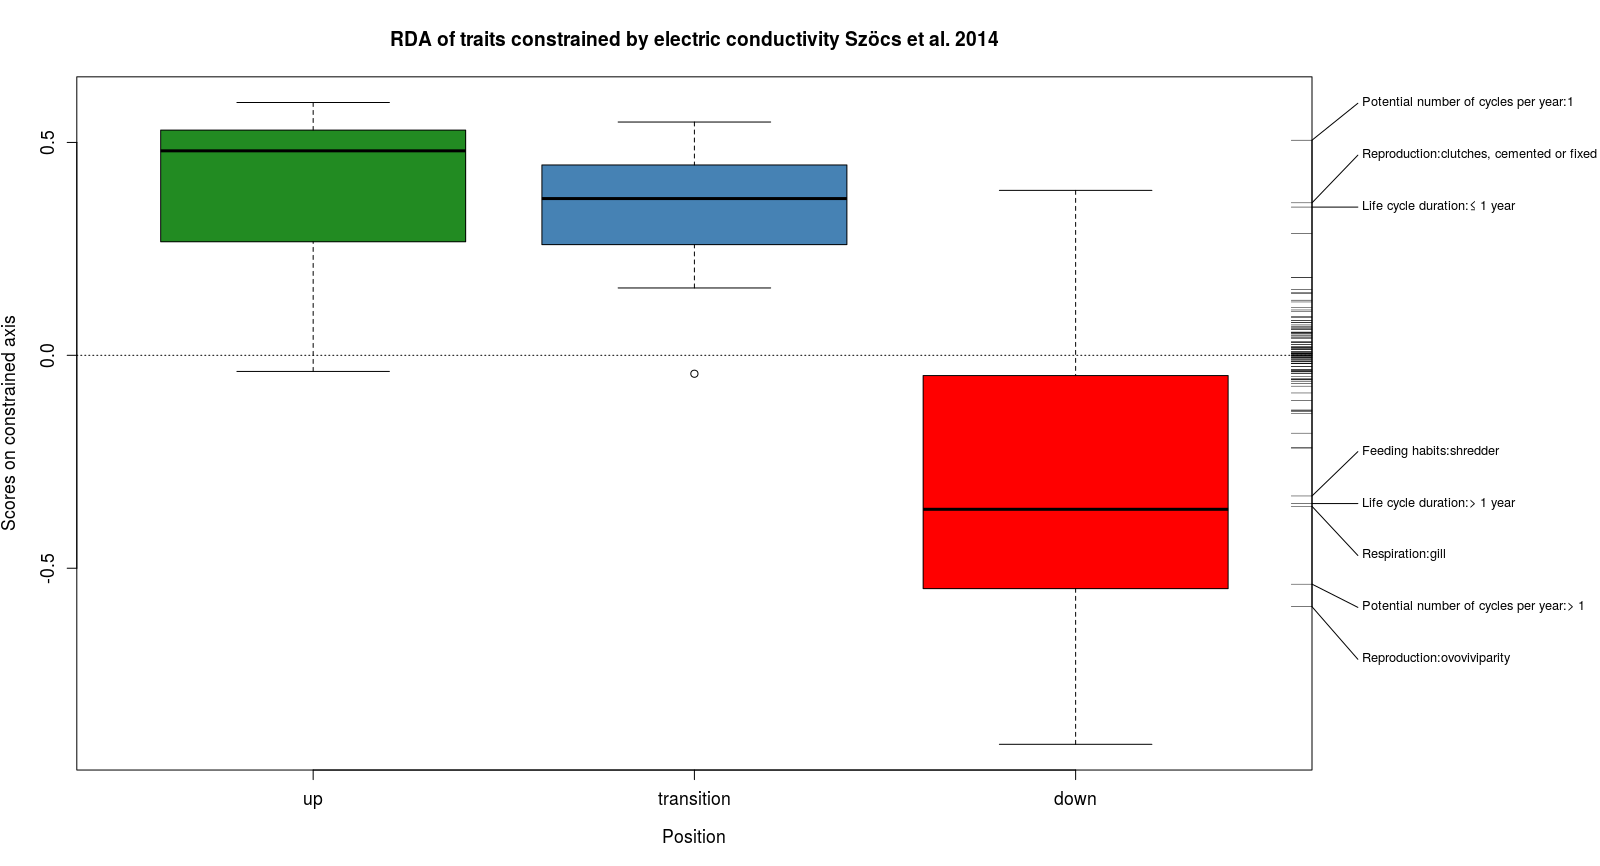
\includegraphics[width=16.5cm, height=10cm]{RDA_traits_Szoecs_2014.png}
%     \caption{RDA of traits constrained by electric conductivity. Boxplot of site scores along the conductivity axis ($30.09 \%$ explained variance, p = 0.001, 1000 permutations). Rug on the right indicates trait scores on the conductivity axis. Only traits with a mahalanobis distance greater than 5.02 were labeled.
%     } 
% \end{figure}

% Not sure if the next two sections are really needed
% Need also to run analysis again
%\subsubsection*{Trait distribution along first RDA axis} 

% \begin{figure}[H]
%     \centering
%     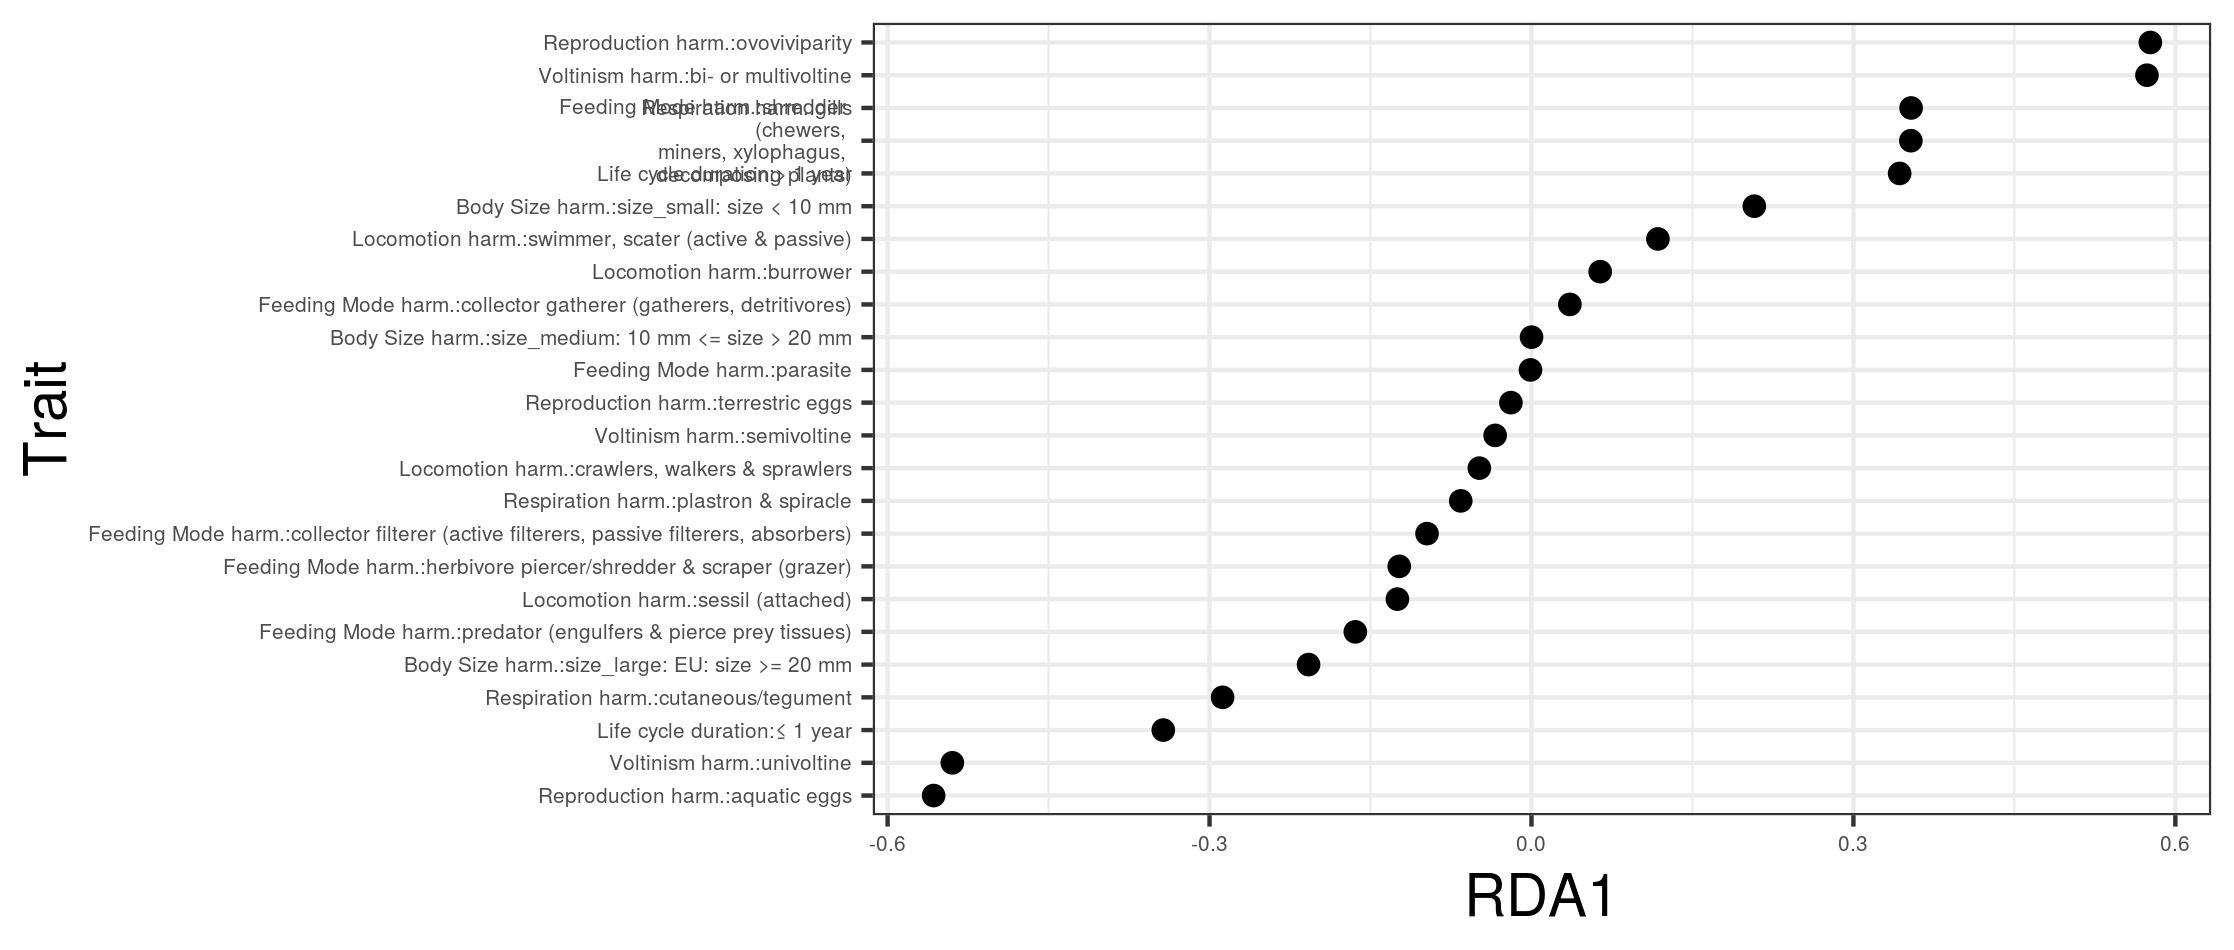
\includegraphics[width=17.5cm, height=10cm]{Trait_distrb_harmonized.png}
%     \caption{Trait scores on the first RDA axis for harmonized traits and traits of the grouping feature \textit{life cycle duration}.
%     } 
% \end{figure}

% \begin{figure}[H]
%     \centering
%     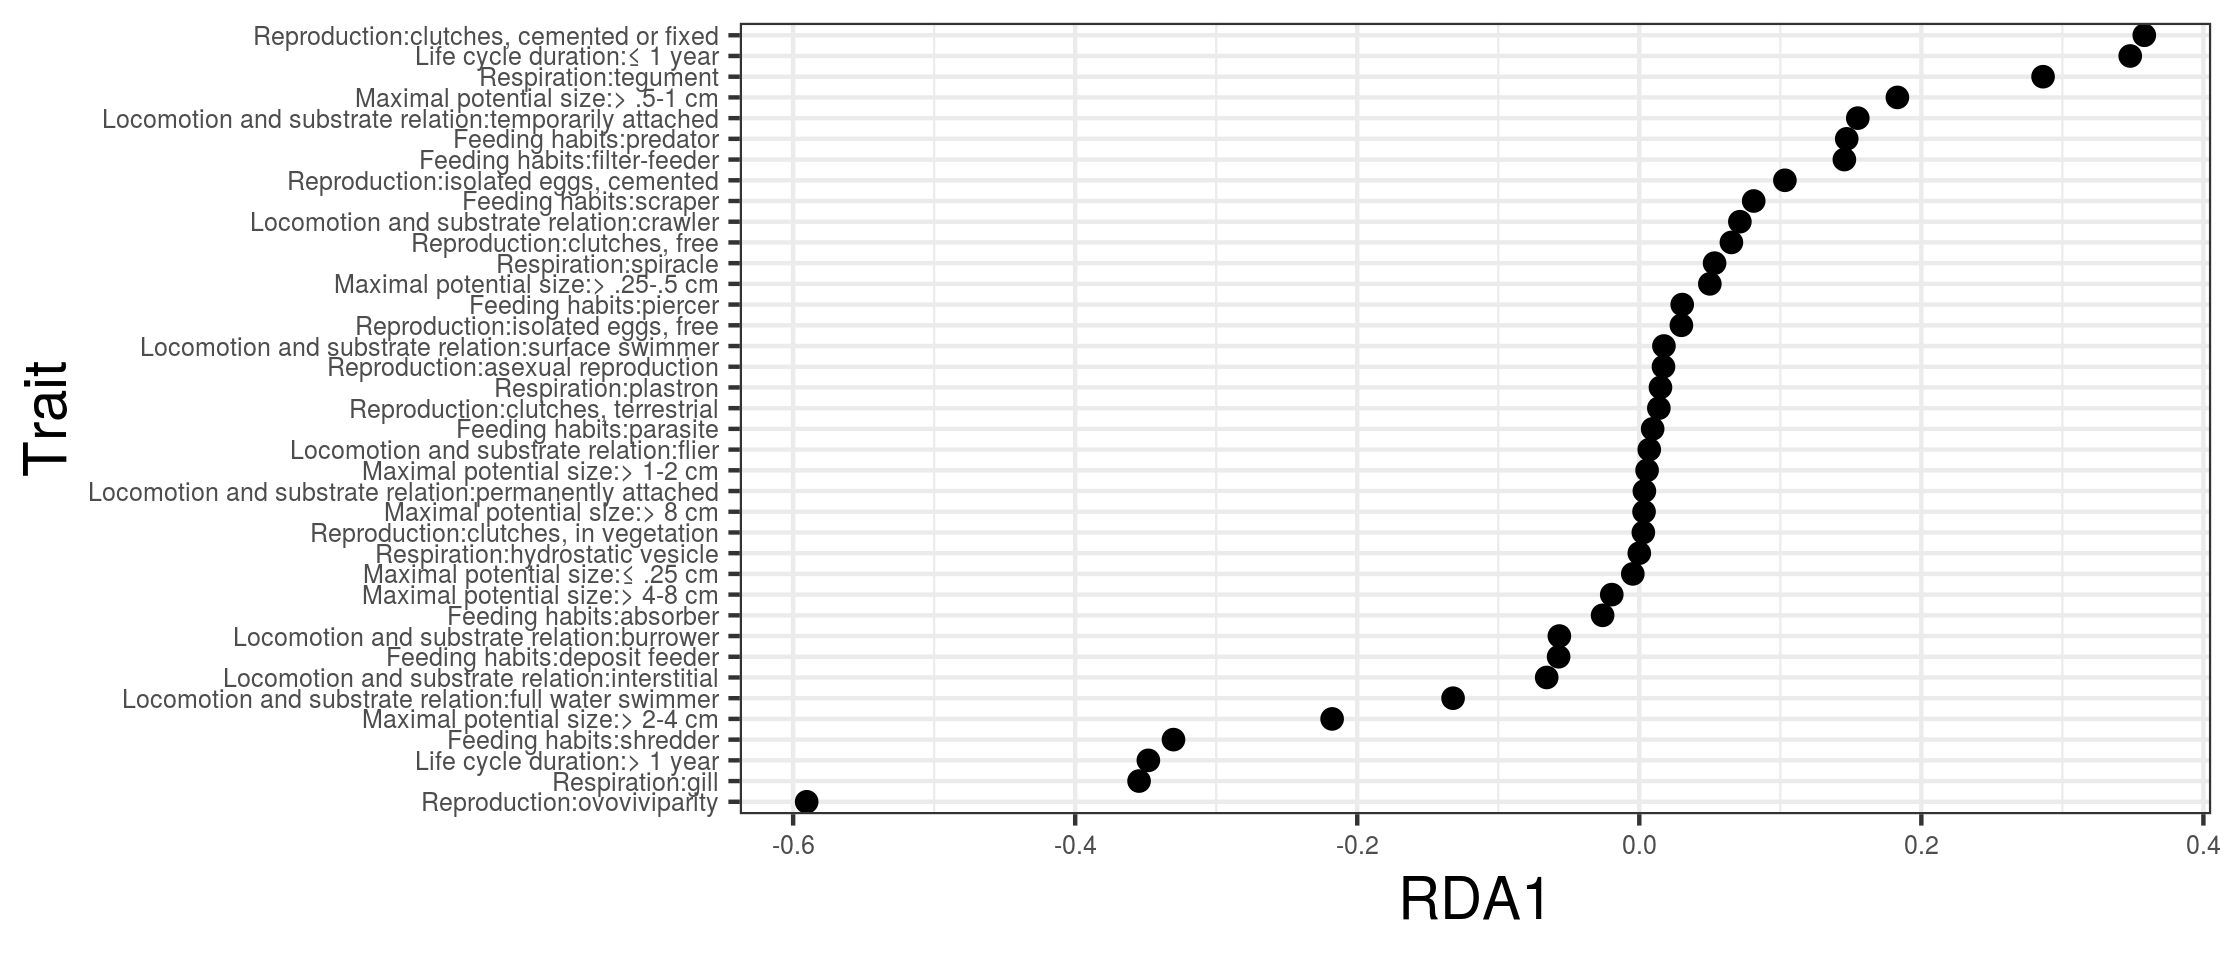
\includegraphics[width=17.5cm, height=10cm]{Trait_distrb_Szoecs_2014.png}
%     \caption{Trait scores on the first RDA axis for the traits responding to high salinity in Szöcs et al. \cite{szocs_effects_2014}
%     .
%     }
% \end{figure}

\newpage
% \subsubsection*{Linear models of trait proportions}

% \textit{Linear models of trait proportions with harmonized traits:}
% \begin{table}[ht]
%     \centering
%     \caption{Results of linear models for the four selected harmonized traits and life cycle duration $>$ 1 year. Trait proportions were logit transformed prior model building, estimates are on the logit scale. Although years were statistically not significant we kept this factor in the model to avoid temporal autocorrelation. Bold values indicate statistically significant effects (p $<$ 0.05).}
%     \label{stab:linear_models_new}
%     \begin{tabular}{l|ccccc}
%     \toprule[.1em]
%     & \specialcell{Feeding mode:\\ shredder} & \specialcell{Life cycle duration:\\ $>$ 1 year} & \specialcell{Voltinism:\\ bi- or multivoltine} & \specialcell{Reproduction:\\ ovoviviparity} & \specialcell{Respiration:\\ gills} \\ 
%     \toprule[.1em]
%     Intercept ($=$ upstream) & \textbf{-1.041} & \textbf{-0.486} & 0.375* & \textbf{-0.823} & 0.092\\ 
%     Downstream & \textbf{0.926} & \textbf{0.605} & \textbf{1.376} & \textbf{1.684} & \textbf{0.854}\\ 
%     Downstream x 2008 & -0.117 & 0.106 & -0.235 & -0.088 & -0.317\\ 
%     Downstream x 2009 & 0.030 & -0.056 & 0.001 & 0.245 & 0.180\\ 
%     Year 2008 & -0.167 & -0.115 & 0.033 & -0.182 & -0.151\\ 
%     Year 2009 & 0.175 & 0.086 & -0.088 & 0.246 & 0.141\\ 
%     \bottomrule
%     \end{tabular}
%     \textit{* p.value = 0.055}
% \end{table}
% \newline
% \newline
% \newline
% \textit{Linear models of trait proportions Szöcs et al. :}
% \begin{table}[ht]
%     \centering
%     \caption{Results of linear models for the five selected traits for Szöcs et al. \cite{szocs_effects_2014}. Trait proportions were logit transformed prior model building, estimates are on the logit scale.
%     Although years were statistically not significant we kept this factor in the model to avoid temporal autocorrelation. Bold values indicate statistically
%     significant effects (p $<$ 0.05).}
%     \label{stab:linear_models_edi}
%     \begin{tabular}{l|ccccc}
%     \toprule[.1em]
%     & \specialcell{Feeding habits:\\ shredder} & \specialcell{Life cycle duration:\\ $>$ 1 year} & \specialcell {Cycles per year:\\ $>$ 1} & \specialcell{Reproduction:\\ ovoviviparity} & \specialcell{Respiration:\\ gills} \\ 
%     \toprule[.1em]
%     Intercept ($=$ upstream) & \textbf{-0.853} & \textbf{-0.478} & \textbf{0.603} & \textbf{-0.838} & 0.111 \\ 
%     Downstream & \textbf{0.819} & \textbf{0.594} & \textbf{1.297} & \textbf{1.679} & \textbf{0.839} \\ 
%     Downstream x 2008 & -0.155 & 0.102 & -0.227 & -0.070 & -0.314 \\ 
%     Downstream x 2009 & 0.073 & -0.053 & -0.020 & 0.248 & 0.176 \\ 
%     Year 2008 & -0.122 & -0.112 & 0.026 & -0.192 & -0.154 \\ 
%     Year 2009 & 0.167 & 0.084 & -0.104 & 0.250 & 0.139 \\ 
%     \bottomrule
%     \end{tabular} 
% \end{table}


% \subsubsection*{Trait proportions over time}
% \begin{figure}[H]
%     \centering
%     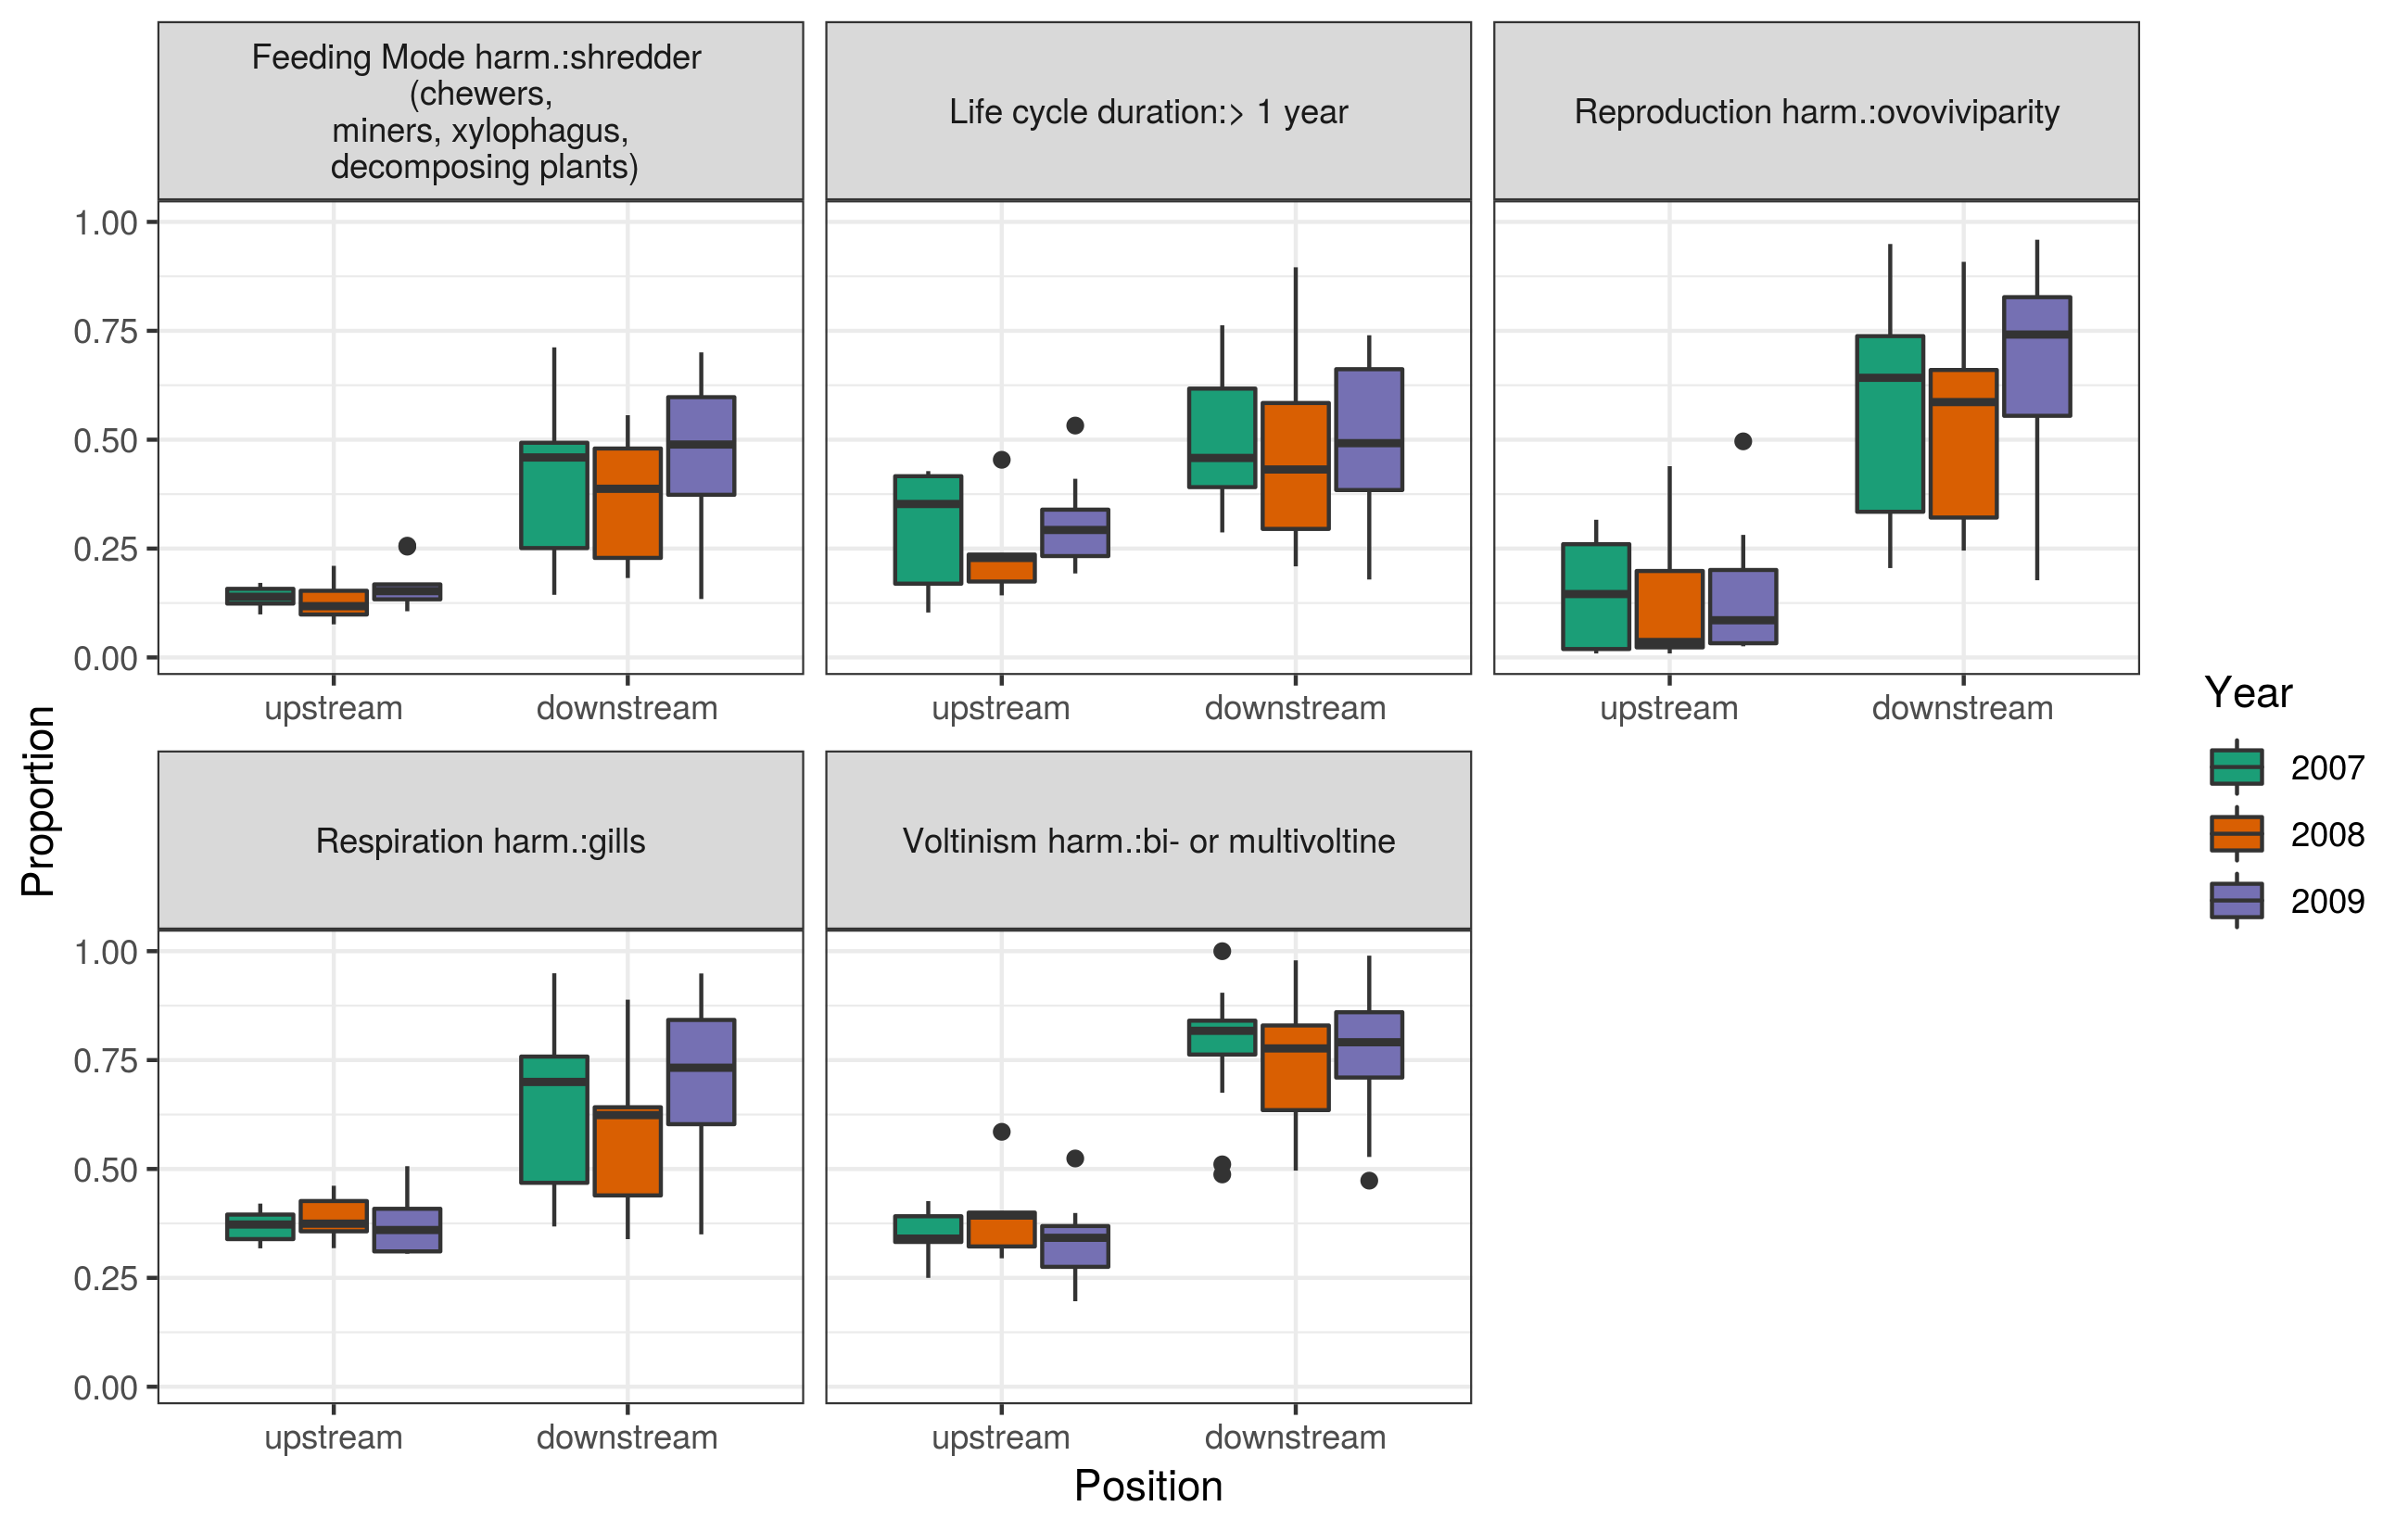
\includegraphics[width=16.5cm, height=10cm]{Trait_proportion_harmonized.png}
%     \caption{Proportions for the four harmonized traits that have been promoted by salinization and life cycle duration $>$ 1 year for down- and upstream sites.
%     } 
% \end{figure}

% % Trait proportions over time
% \begin{figure}[H]
%     \centering
%     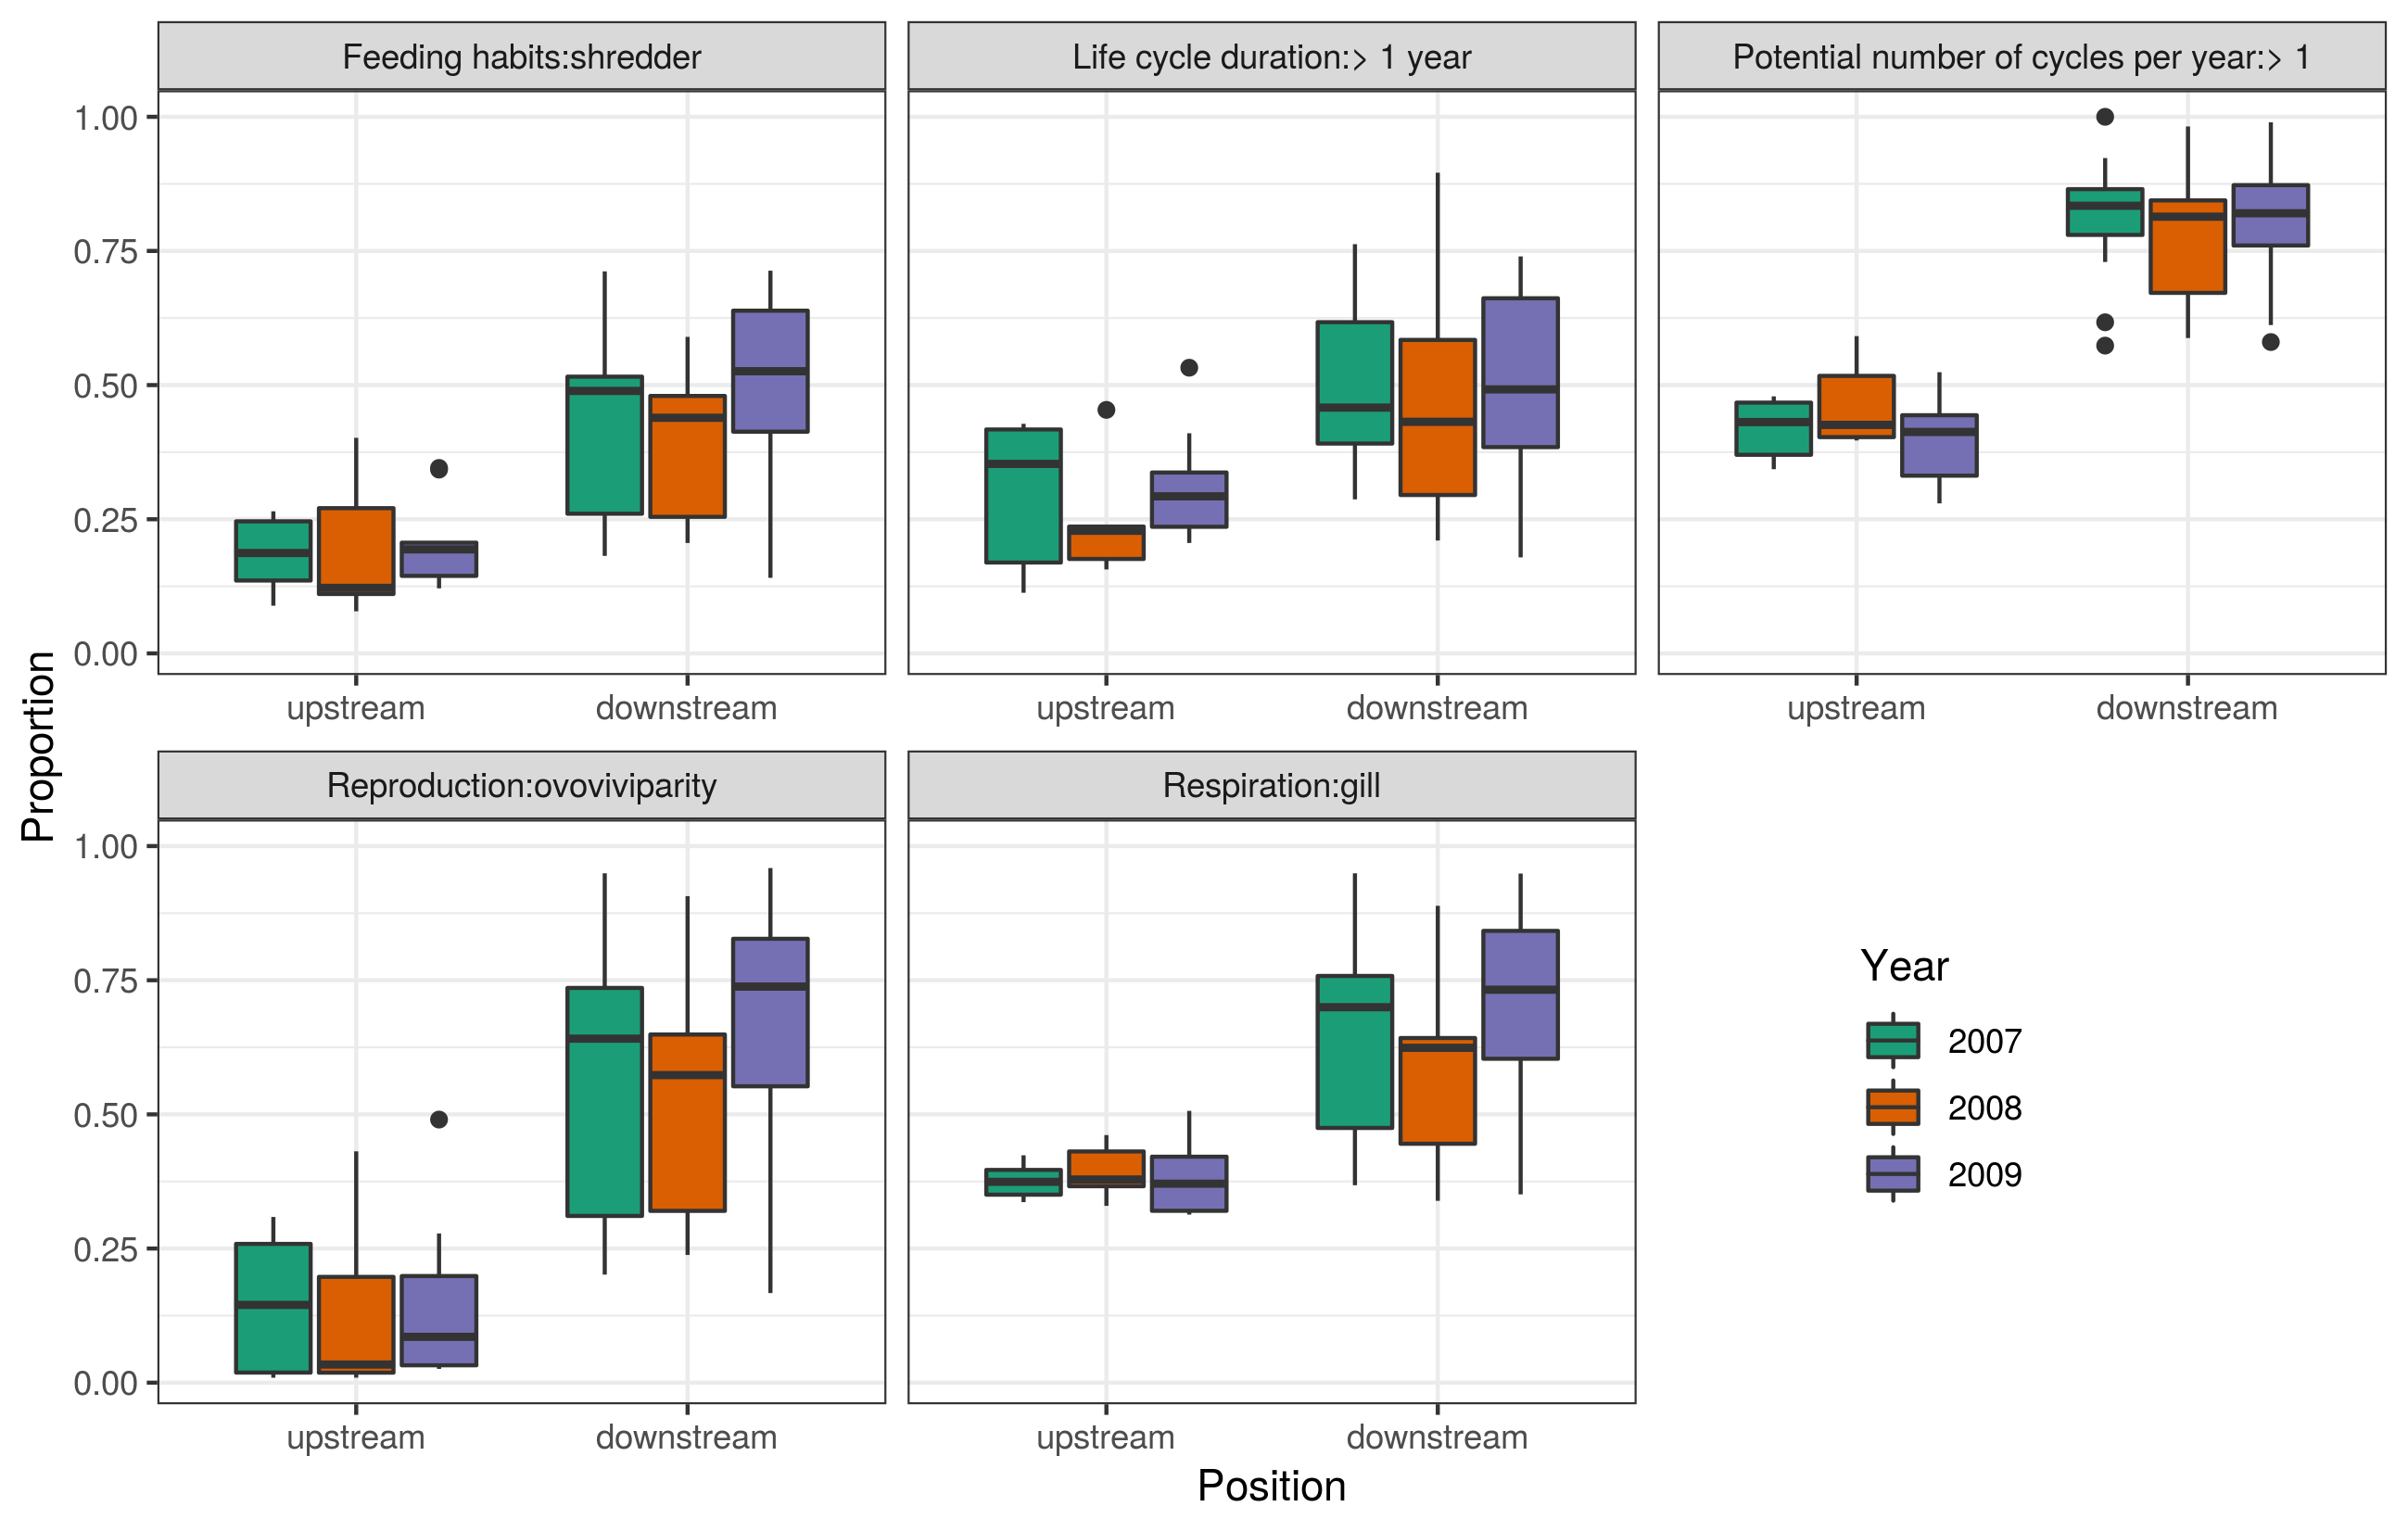
\includegraphics[width=16.5cm, height=10cm]{Trait_proportion_Szoecs_2014.png}
%     \caption{Proportions for five selected traits for down- and upstream sites (traits that have been promoted by salinization) from Szöcs et al. \cite{szocs_effects_2014}.} 
% \end{figure}




\end{document}